%\newcommand{\eps}{\epsilon}
\newcommand{\Pmax}{p_\text{max}} 	
\newcommand{\Hint}{H_{int}}
\newcommand{\kbar}{\bar{k}}
\newcommand{\Delk}{\Delta}
\newcommand{\Sumk}{\Sigma}
\newcommand{\Qrot}{Q_{pq}(\tau_s)}
\newcommand{\shapecor}{\mathcal{S}}
\newcommand{\ampcor}{\mathcal{A}}
\newcommand{\totalcor}{\mathcal{E}}
\newcommand{\threeLs}{L_p(\kbar_1)L_q(\kbar_2)L_r(\kbar_3)}
\newcommand{\threePs}{P_p(\kbar_1)P_q(\kbar_2)P_r(\kbar_3)}
\newcommand{\threeQs}{Q_p(k_1)Q_q(k_2)Q_r(k_3)}
\newcommand{\Lbasic}{\mathcal{P}_0}
\newcommand{\Linvk}{\mathcal{P}_1}
\newcommand{\Lnsinv}{\mathcal{P}^{n_s}_1}
\newcommand{\Lnsboth}{\mathcal{P}^{n_s}_{01}}
\newcommand{\Linvksq}{\mathcal{P}_2}
\newcommand{\Lns}{\mathcal{P}^{n_s}_2}
\newcommand{\Fbasic}{\mathcal{F}_0}
\newcommand{\Finvk}{\mathcal{F}_1}
\newcommand{\Finvksq}{\mathcal{F}_2}
\newcommand{\quadpot}{V_{\phi^2}(\phi)}
%\newcommand{\threeqs}{q_p(\kbar_1)\,q_r(\kbar_2)\,q_s(\kbar_3)}
\newcommand{\threeqs}{q_p(k_1)\,q_r(k_2)\,q_s(k_3)}
\newcommand{\threeqstilde}{q_{\tilde{p}}(k_1)\,q_{\tilde{r}}(k_2)\,q_{\tilde{s}}(k_3)}
\newcommand{\kmin}{{k_\text{min}}}
\newcommand{\kmax}{{k_\text{max}}}
\newcommand{\fnl}{f_{NL}}
\newcommand{\fnllocal}{f^{local}_{NL}}
\newcommand{\fnlequil}{f^{equil}_{NL}}
\newcommand{\fnlortho}{f^{ortho}_{NL}}

\chapter{Decomposing Primordial Shapes}\label{chapter:decomp}
As we have seen, while at tree level the bispectrum is an integral
over a separable integrand (see~\eqref{inin_integral} and
the example presented in~\eqref{inin_computer}),
this separability is usually lost
in the final result. In this chapter we outline a formalism that preserves the
separability, by expanding the integrand in a separable basis. We also explore
possible choices for this separable basis, testing them on various
shape functions from the literature and highlighting the choices with
sufficiently fast and broad convergence to be useful in realistic
inflationary parameter scans.


\section{Setting up the formalism}\label{sec:setting_notation}
Given its separable form, the tree-level in-in formalism is amenable
to more efficient calculation using separable modes, as first mentioned in~\cite{Funakoshi}.
That work extended the separable methodology previously implemented for the CMB
bispectrum~\cite{FergShell_1,FergShell_2,FergShell_3}.
Our goal in this work is the efficient calculation of more general bispectra
which may have significant (possibly oscillatory) features, requiring searches across inflationary parameters.
To achieve this, we represent the shape function~\eqref{shapefn} using a set of basis functions as
\begin{align}\label{goal}
S(k_1, k_2,k_3) &= \sum_n \alpha_n  \, Q_n(k_1,k_2,k_3)\,,
\end{align}
where the basis functions $Q_n(k_1,k_2,k_3)$ are explicitly separable functions of their arguments.
The specific bispectrum information of each scenario is encoded in $\alpha_n$.
Translating this result into a constraint from the CMB
will require a large once-off computational cost---however, this cost will be
paid once per set of basis functions $Q_n$, not per scenario.
The details of this once-per-basis calculation will be
presented in~\cite{Sohn_2021}.
As such, while the general computational steps we
describe will be independent of the basis, it is vital we
explore possible sets of basis functions $Q_n(k_1,k_2,k_3)$
and their effects on convergence;
that will be the main subject of this chapter.
In this section we will set the notation we will use to recast
the standard numerical in-in calculation into a calculation of $\alpha_n$ in~\eqref{goal}.
We will sketch the steps involved, including accounting for the effect of spatial derivatives
in the interaction Hamiltonian on our final result.
The rest of this chapter is then devoted to developing and comparing possible basis sets.
In chapter~\ref{chapter:methods} we will then use the formalism and the basis sets of this chapter to
make precise the numerical considerations of the calculation,
especially our methods of dealing with the high-frequency
oscillations at early times.


The values of the coefficients $\alpha_n$ will depend on the choice
of basis, but the methods we will describe to calculate them
will be practical for any basis.
Our aim will be to separate out the dependence on $k$ and $\tau_s$,
without losing any of the information contained in the tree-level in-in formalism,
except in the sense that is controlled by $\Pmax$.
We will set up an efficient numerical implementation of the calculation,
a necessary consideration to allow this method to be useful in exploring
parameter spaces in primordial phenomenology.
Throughout we will see that we are able to preserve the
separability of the dependence on $k_1$, $k_2$ and $k_3$.


The tree-level in-in formalism for the bispectrum~\eqref{inin_integral} is inherently separable given
the form of the cubic interaction Hamiltonian $H_{\rm int}$.
This can be clearly seen in the integrand of the example in~\eqref{inin_computer}.
Consider indexing with ${i=1,2,3...}$ the interaction vertices in $H_{\rm int}$,
so then after the contractions have been performed,
the bispectrum~\eqref{inin_integral} can be expressed as a sum over separable contributions of the form:


\begin{align}\label{inin_sep}
    S(k_1, k_2,k_3) &= \sum_i I^{(i)} (k_1, k_2,k_3)\nonumber \\
    &= \Re\sum_i \bigg[ v^{(i)}(k_1, k_2,k_3) \int^0_{-\infty(1-i\varepsilon)} d\tau\, w^{(i)}(\tau) F^{(i)}(\tau,k_1)\, G^{(i)}(\tau,k_2)\,J^{(i)}(\tau,k_3)\nonumber\\
    &\quad\quad\quad\quad\quad\quad\quad\quad\quad\quad+ \text{cyclic perms}  \bigg] 
\end{align}
where $w^{(i)}(\tau)$ is a function of the scale factor and the other background parameters~\eqref{slowrollparams} for the $i$-th interaction vertex, while the terms $F^{(i)}, G^{(i)}, J^{(i)}$ are given by the Fourier mode functions $k^2\zeta_{k}(0)\zeta^{*}_{k}(\tau)$ or their time derivatives $k^2\zeta_{k}(0)\dzeta^{*}_{k}(\tau)$.
Spatial derivative terms also separate because of the triangle condition~\eqref{triangle_condition}.
For example, a term such as  $\partial_i \zeta\, \partial_i\zeta$ becomes
$(-{\bf k_2}\cdot {\bf k_3} )\zeta_{{k}_2}(\tau)\, \zeta_{{k}_3}(\tau)$.
Since  ${\bf k_2}\cdot {\bf k_3} = (k_1^2 - k_2^2-k_3^2)/2$, this yields a sum of separable terms.
These time-independent contributions are contained in $v^{(i)}(k_1, k_2,k_3)$,
as they do not force us to compute extra time integrals.
Note that $v^{(i)}(k_1, k_2,k_3)$ need not be symmetric in its arguments.


We can connect this form to the example given in~\eqref{inin_computer}.
In that example, we see there is no sum over $i$ as we took only one term of $\Hint$.
We also see that $v^{(i)}(k_1,k_2,k_3)=1$ as there are no spatial derivatives.
Collecting the terms with no $k$ dependence, we see that
$w^{(i)}(\tau)=-2ig(\tau)a^4(\tau)$.
The remaining terms then give
\begin{align}
    F^{(i)}(\tau,k) = G^{(i)}(\tau,k) = J^{(i)}(\tau,k) = k^2\zeta_k(0)\dzeta_k^*(\tau)
\end{align}
where the $k^2$ comes from the definition of the shape function~\eqref{shapefn},
and we obtain $\zeta_k(\tau)$ by numerically solving the equation of motion~\eqref{modefneqn_zeta_N}.


The terms contained in $v^{(i)}(k_1, k_2,k_3)$ depend on the structure of the spatial derivatives in the interaction Hamiltonian,
but not the specific scenario. These terms are separable;
we will discuss their precise form in section~\ref{sec:h_int}.
We include their contribution to the final result after the time integrals have been computed.
The factors which depend only on time, $w_i(\tau)$, depend on the scenario
but do not need to be decomposed in $k$.
The remaining factors have both $k$ and time dependence;
they must be decomposed in $k$ at every timestep.
As we have mentioned, these terms look like $F^{(i)}(k, \tau) = k^{2} \zeta_{\bf k}(0)\zeta_{\bf k}^*(\tau)$,
with a possible time derivative.
The factor of $k^2$ could be absorbed into $v^{(i)}(k_1, k_2,k_3)$, but we have the freedom to keep it here to aid convergence.

If the expressions being expanded have some known pathology in their $k$-dependence,
we can then see two ways of dealing with this.
The basis can be augmented to efficiently capture the relevant behaviour
(as we will explore in the rest of this chapter)
or the behaviour can be absorbed into the analytic prefactor, $v^{(i)}(k_1, k_2,k_3)$.\footnote{At early times the modes are highly oscillatory in both $k$ and $\tau_s$, to which we will certainly give special attention.}
We use the former, as the numerics of the latter are less transparent
and less physically motivated.

The internal basis used for the decomposition at each timestep need not match that
which is used for the final result,
and indeed in dealing with the spatial derivatives in section~\ref{sec:h_int}
we will find it useful to change to a different basis than the one used to perform the
time integrals of the decompositions.

\textcolor{red}{Jarring, move earlier.}
Using the approximate mode functions~\eqref{modefnsapprox}, an explicit example for the first interaction term in~\eqref{interaction_loc}, i.e.\ $H_{\rm int}^{(1)} = {\zeta'}^2\zeta$, takes the form
\begin{align}\label{inin_example_FG}
    F^{(1)}(\tau,k) = G^{(1)}(\tau,k)  ~&=~  c_s k^2 \tau\frac{H^2}{4\varepsilon c_s} e^{ic_{\rm s} k\tau}~,\\
    J^{(1)}(\tau,k) ~&=~ (1-ik c_{\rm s}\tau)\frac{H^2}{4\varepsilon c_s}e^{ic_{\rm s} k\tau} \,.
\end{align}
In the simple mode approximation~\eqref{modefnsapprox}, such terms in~\eqref{inin_sep} are straightforward to integrate analytically (using the $i\varepsilon$ prescription), provided the time-dependence of the slow-roll parameters and the sound speed is neglected~\cite{Maldacena}.
However, for high precision bispectrum predictions we must incorporate the full time-dependence,
while solving~\eqref{modefneqn_zeta_N} to find accurate mode functions $\zeta_{\bf k}(\tau)$ numerically.
Obtaining the full 3D bispectrum directly is computationally demanding at high resolution because
it requires repetitive integration of~\eqref{inin_sep} at each specific point for the wavenumbers $(k_1, k_2, k_3)$,
a problem which is drastically compounded by bispectrum parameter searches e.g.\ for oscillatory models. 


We will now link~\eqref{inin_sep} to~\eqref{goal}.
Consider representing the primordial shape function $S(k_1, k_2, k_3)$ in~\eqref{inin_sep} as
a mode expansion for each interaction term $I^{(i)}(k_1, k_2,k_3)$ as
\begin{align}\label{modeexp}
S(k_1, k_2,k_3) &= \sum_i I^{(i)}(k_1,k_2,k_3) =  \sum_i \sum_n \alpha_n^{(i)}  \, Q_n(k_1,k_2,k_3)\,,
\end{align}
where $Q_n(k_1,k_2,k_3)$ is separable, built out of some
orthonormal set $q_p(k)$ as in~\eqref{modes3d}.
Armed with this set of modes,
we can expand any of the interaction terms $F^{(i)}(\tau, k)$, $G^{(i)}(\tau, k)$, $J^{(i)}(\tau, k)$
in~\eqref{inin_sep} as:
\begin{align}
    F^{(i)}(\tau, k) &= \sum _p f_p^{(i)} (\tau) \, q_p(k)\,,\label{mode1Dcoeffs_sum}\\
    \text{where} \quad f_p^{(i)} (\tau)  &= \int _\kmin^\kmax dk \,F^{(i)}(\tau, k) \, q_p(k) \,.\label{mode1Dcoeffs_integral}
\end{align}


Substituting these expansions into~\eqref{inin_sep}, we obtain the following decomposition for the $i$-th vertex contribution,
\begin{align}\label{inin_kdep}
    &I^{(i)}(k_1,k_2,k_3)
    = \Re\bigg[v^{(i)}(k_1, k_2,k_3)\int^0_{-\infty(1-i\varepsilon)} d\tau\, w^{(i)}(\tau)\nonumber\\
    &\qquad\cdot\sum_p f_p^{(i)}(\tau) q_p(k_1)\sum_r g_r^{(i)}(\tau) q_r(k_2)\sum_s h_s^{(i)}(\tau) q_s(k_3) + \text{cyclic perms}\bigg]\\
	&= v^{(i)}(k_1, k_2,k_3)\sum_{prs}\bigg(\Re\int^0_{-\infty} d\tau\, w^{(i)}(\tau)\nonumber\\
    &\qquad\qquad\cdot f_p^{(i)}(\tau)\, g_r^{(i)}(\tau) \,h_s^{(i)}(\tau)\bigg)\threeqs + \text{cyclic perms}\,.
\end{align}
For the sake of compactness of notation we use $P$ to stand for the
triplet $p,r,s$ and $\tilde{P}$ to stand for the triplet $\tilde{p},\tilde{r},\tilde{s}$.
Note that we have dropped the $i\varepsilon$ prescription---this is due to the fact that the
integrals are now convergent, as pointed out in~\cite{Funakoshi}, and as we discuss in section~\ref{sec:starting}.
Writing $q_{P}(k_1,k_2,k_3)=\threeqs$,
we continue,
\begin{align}\label{inin_kdep_cont}
    I^{(i)}(k_1,k_2,k_3) =&\, v^{(i)}(k_1, k_2,k_3) \sum_{P} \tilde{\alpha}_{P}^{(i)}\,  q_{P}(k_1,k_2,k_3) + \text{cyclic perms}\nonumber\\
    =& \sum_{P} \tilde{\alpha}_{P}^{(i)}\sum_{\tilde{P}}V^{(i)}_{P\tilde{P}}\,  q_{\tilde{P}}(k_1,k_2,k_3) + \text{cyclic perms}\nonumber\\
    =& \sum_{\tilde{P}} \alpha_{\tilde{P}}^{(i)}\,  q_{\tilde{P}}(k_1,k_2,k_3) + \text{cyclic perms} \,,
\end{align}
where we have written
\begin{align}\label{inin_kindep}
\tilde{\alpha}_P^{(i)} =  \tilde{\alpha}_{prs}^{(i)} 	= \Re\int^0_{-\infty} d\tau\, w^{(i)}(\tau)\, f_p^{(i)}(\tau) \,g_r^{(i)}(\tau) \,h_s^{(i)}(\tau)\,,
\end{align}
and included the time-independent $k$-prefactors from the interaction Hamiltonian by writing
\begin{align}\label{V_definition}
    v^{(i)}(k_1, k_2,k_3)q_P(k_1,k_2,k_3) = \sum_{\tilde{P}}V^{(i)}_{P\tilde{P}}q_{\tilde{P}}(k_1,k_2,k_3)\,,
\end{align}
and
\begin{align}
    \alpha_P^{(i)} = \sum_{\tilde{P}} \tilde{\alpha}_{\tilde{P}}^{(i)}V^{(i)}_{\tilde{P}P} + \text{cyclic perms}.
\end{align}
%We connect to the coefficients of the ordered, symmetrised basis in~\eqref{modeexp} by taking the symmetry factor into account,
%\begin{align}
%    \alpha_n^{(i)} = \frac{3!}{\Xi_P}\alpha_P^{(i)}.
%\end{align}
The numerical calculation of $V^{(i)}_{P\tilde{P}}$ (as defined by~\eqref{V_definition}) is highly efficient as $v^{(i)}(k_1, k_2,k_3)$
is a sum of separable terms. The details of these terms
depend only on the spatial derivatives in the interaction Hamiltonian, not the scenario being
considered, so the matrix can be precomputed and stored.
Note that this is not the only way one can organise this calculation to
explicitly preserve the separability. One could also include the contributions
coming from the spatial derivatives first, decomposing (as in~\eqref{mode1Dcoeffs_sum}) not only terms
like $k^{2} \zeta_{\bf k}(0)\zeta_{\bf k}^*(\tau)$, but also terms that include
each power of $k_1$, $k_2$ or $k_3$ that appears in $v(k_1,k_2,k_3)$. The index $i$
in the sum in~\eqref{modeexp} would then run over not only each vertex in the interaction
Hamiltonian, but also each separable term within those vertices.
We do not choose this path as, for the sake of efficiency, we wish to minimise the
number of time integrals of the form~\eqref{inin_kindep} we need to calculate.


Note the basis sets on the left and right hand side of~\eqref{V_definition}
need not match. In fact, if those two basis sets do match, then generically information
will be lost---for example, if the basis set on the left is $\Lbasic$, then terms
in $v^{(i)}(k_1,k_2,k_3)$ with positive powers will introduce higher order
dependencies on $k$, and negative powers will introduce $1/k$ behaviour. In
practice, to prevent this loss of information, we take the basis set on the right hand
side of~\eqref{V_definition} to be an expanded version of that on the left. For
example, if the left hand basis was $\Lbasic$ of size $\Pmax$, the right hand basis would
be $\Linvk$ of size $\Pmax+3$.


We can see from~\eqref{inin_kindep} that the number of time integrals needed is controlled by
$N_V\times\Pmax^3$\footnote{In fact the number is not quite $\Pmax^3$.
Since we have extracted the spatial derivatives, the only remaining
possible source of asymmetric $k$-dependence
comes from $\zeta^3$, $\zeta^2\zeta'$, $\zeta'^2\zeta$ or $\zeta'^3$
so the time integral in~\eqref{inin_kindep} will always be (at least) symmetric in $p$ and $r$. },
where $N_v$ is the number of interaction vertices
and $\Pmax$ is the size of the basis.
Since the calculational cost of doing the internal decompositions depends only
linearly on the size of internal basis, improvements there are dwarfed by improvements
gained from reducing the number of terms needed in the final basis.


Having calculated the contribution of each $\Hint$ vertex separately,
indexed as above by $(i)$, the overall shape function~\eqref{modeexp} is then simply
\begin{align}\label{shapemodeexp}
    S(k_1, k_2,k_3) =   \sum_n \left(\sum_i \alpha_n^{(i)}\right) \, Q_n(k_1,k_2,k_3) =  \sum_n \alpha_n \, Q_n(k_1,k_2,k_3) \,.
\end{align}
Depending on the scenario,  some vertex contributions will converge faster than others 
or be completely negligible;
for efficiency the maximum modal resolution defined by $\Pmax$ can be allowed to be different
for each vertex.  
 

It is worth emphasising that the raison d'etre for this approach is that all time integrals~\eqref{inin_kindep} are now independent of the $k$-configuration\footnote{
    They are not independent of $\kmin$ and $\kmax$ which define the domain of interest,
    which is analogous to the coefficients of a Taylor expansion depending on its expansion point.
}.
In a configuration-by-configuration method one improves the precision by
decreasing the spacing which defines the density of the grid of points within the tetrapyd.
Instead, in the modal approach, we increase precision by adding more modes to the shape function expansion~\eqref{shapemodeexp}
until the result converges at high precision.   At first sight, this appears to increase the dimensionality of the calculation.
Directly integrating the in-in formalism requires one time
integration for each $k$-configuration, i.e. $N_k^3$ integrals, ignoring symmetry.
The method detailed here requires decomposing the modes,
then a time integral for every coefficient, i.e. $\Pmax^3$ integrals
(again ignoring symmetry) in addition to the decomposition.
However for every model we have explored from the literature,
our expansion in $\Pmax$ converges far faster than in the number of
$k$-modes that would be required to have confidence in a sampled bispectrum.
This is clear in smooth bispectra such as~\eqref{malda_shape} and~\eqref{dbi_shape},
but is also true of bispectra with complicated features,
as quantified by the figures later in this chapter.


To be efficiently connected to a late-time observable
a sampled bispectrum would have to be fit by a smooth template,
a complication that is automatically taken care of in this formalism.
We note that the primordial basis can be chosen
independently of the final bispectrum basis employed for observational tests---a change of
basis $Q_{pqr}\rightarrow \tilde Q_{pqr}$ can be trivially
and cheaply achieved through a linear transformation $\Gamma$
with the new expansion coefficients given by $\tilde \alpha_{abc} = \Gamma_{ap}\Gamma_{bq}\Gamma_{cr}\alpha_{pqr}$. 


Discussion of convergence in this chapter is considered only at the primordial level,
with no concept of the signal to noise of an actual experiment.
There could be a basis that converges faster in some observationally weighted sense,
efficiently describing the primordial modes which will matter most at late times.
We leave discussion of this point to a later work, as converting between the two,
after the in-in computation is completed, is trivial.


Having now set our notation and outlined the calculation, in the following sections we
discuss possible basis sets, before presenting the details on
the numerical implementation of these methods in chapter~\ref{chapter:methods}.


\section{Testing basis sets}\label{sec:inner_product}
We define the inner product of two bispectrum shape functions as
\begin{align}
    S_1\cdot S_2  = \langle S_1\,, S_2 \rangle = \int_{T_k} d^3k \: S_1(k_1,k_2,k_3) \: S_2(k_1,k_2,k_3)\,,\label{inner_prod}
\end{align}
where $T_k$ refers to the tetrapyd, the region of the cube $[\kmin,\kmax]^3$ that obeys the triangle inequality.
Following~\cite{hung_1902}
we define the two correlators:
\begin{align}
    \shapecor(S_1,S_2) = \frac{S_1\cdot S_2}{\sqrt{(S_1\cdot S_1)(S_2\cdot S_2})}\,, \qquad\quad 
\ampcor(S_1,S_2) = \sqrt{\frac{S_1\cdot S_1}{S_2\cdot S_2}}\,.
\end{align}
Here, we refer to $\shapecor(S_1,S_2)$ as the shape correlator between the two bispectra;
$\ampcor(S_1,S_2)$ is the amplitude correlator.
In principle, we could add some observationally motivated weighting
to the above measure, as considered in~\cite{FergShell_1,FergShell_2,FergShell_3},
but in this work we restrict ourselves to accurately calculating the
full primordial bispectra, weighting each configuration equally.

Writing $|S|^2=S\cdot S$,
we can then re-express a measure of the relative error
between one bispectrum template and another:
\begin{align}\label{relative_difference}
\totalcor(S_1,S_2) &= \sqrt{\frac{|S_1-S_2|^2}{|S_2|^2}}  = \sqrt{\frac{|S_1|^2-2S_1\cdot S_2+|S_2|^2}{|S_2|^2}}\nonumber\\
	   &= \sqrt{\ampcor(S_1,S_2)^2-2\ampcor(S_1,S_2)\shapecor(S_1,S_2)+1}.
\end{align}
This error measure takes into account differences in overall magnitude as well as shape.
If we are only interested in comparing the differences coming from the shape,
we can scale the bispectra so that $\ampcor(S_1,S_2)=1$ and so
\begin{align}\label{relative_difference_scaled}
    \totalcor^{(\ampcor=1)}(S_1,S_2) = \sqrt{2(1-\shapecor(S_1,S_2))}.
\end{align}


With this measure of relative difference, a shape correlation of $0.9$ corresponds to a
relative difference of $45\%$,
a shape correlation of $0.99$ corresponds to a relative difference of $14\%$,
a shape correlation of $0.999$ corresponds to a relative difference of $4\%$.
Thus (for our purposes in calculating feature bispectra)
this more exacting measure $\totalcor$ from~\cite{hung_1902} is a far better representation of actual convergence
between two shape functions
than the correlation used in~\cite{Funakoshi}, as it is easier to interpret and
more stringent.


The full relative difference~\eqref{relative_difference} also includes the amplitude
in its measure, which will be important in obtaining an precise link
between fundamental inflationary parameters and the resulting primordial bispectrum.
We will use this measure to test the accuracy and efficiency of our basis expansion
in reconstructing the standard templates, and later to quantify the convergence
of our validation examples in section~\ref{sec:validation}.
In that section we also plot residuals on slices through the tetrapyd,
relative to the representative value
\begin{align}\label{rep_val}
    S^{rep}=\sqrt{\frac{S\cdot S}{\int_{T_k} d^3k}}.
\end{align}


    One degree of freedom that we have not exploited is weighting the decomposition
    to optimise the convergence of the final observable.
    This could be advantageous as it is possible that the CMB could be more sensitive
    to certain $k$-configurations than others, and so we would like those configurations to
    converge most efficiently.
    In this work however we focus on calculating the primordial shape function accurately
    and efficiently and leave exploiting this freedom to a future work.


    An important part of this work is testing the expected convergence of our various
    basis sets on templates of primordial shapes, before testing them in the setting
    of the in-in formalism.
    This testing is important as when testing in the context of the full in-in formalism
    it can be difficult to distinguish between genuine lack of convergence, and
    numerical errors coming from other sources.
    By testing on templates we can estimate the optimal possible
    convergence for a given shape, once all physical effects that contribute
    in the tree-level in-in calculation are taken into account.
    Since the feasibility of our method depends on being able
    to efficiently capture interesting and realistic shapes, this will determine
    which basis sets are worth implementing and testing in the in-in setting.


%\section{The cube and the tetrapyd}
\section{Setting up a basis}
    \subsection{Basis set building blocks}
    Our general strategy will be to start with the Legendre polynomials
    or the Fourier basis functions as a foundation for our basis set.
    We will augment this set with additional basis functions motivated by the
    expected behaviour of primordial shapes in general.
    In this way we can quickly capture the known behaviours,
    but still have the flexibility to converge to a wide range
    of shape functions. It also has the advantage that the Legendre polynomials
    and the Fourier basis functions are automatically orthogonal,
    so we will only have to use the modified Gram–Schmidt process
    (which brings in numerical difficulties)
    a minimal number of times.


    The Legendre polynomials are a basis set with broad descriptive power.
    The Fourier basis functions also have broad descriptive power,
    but are limited by converging poorly to non-periodic functions.
    This problem can be ameliorated through augmenting the basis
    with extra basis functions.


    We augment our basis sets with extra (orthogonalised) basis functions.
    We build these using the more numerically stable modified Gram-Schmidt process,
    orthogonalising the new function with respect to all the basis elements already in
    the basis.


\subsection{Basis choices}\label{sec:large_non_physical}
We now begin our discussion of specific possible sets of separable
basis functions $Q_n(k_1,k_2,k_3)$
for use in the expansion~\eqref{goal}.
Whether the goal is to explore primordial phenomenology or for direct comparison with observations,
the convergence of our basis set will determine the efficiency and practicality
of our methods.
We shall consider constructing the separable basis functions $Q_n(k_1,k_2,k_3)$
out of
%symmetrised
triplet products of normalized one-dimensional modes $q_p(k)$ as
\begin{align}\label{modes3d}
    Q_n(k_1,k_2,k_3)\equiv q_{p} (k_1) \, q_{r}(k_2)\, q_{s}(k_3)\,.
\end{align}
Here, $n$ labels the integer triplet $n \leftrightarrow \{p r s\}$ in some appropriate manner.
%(see some ordering alternatives in~\cite{FergShell_3}), while the symmetrised average of all $\{p r s\}$ permutations is 
%\begin{align}\label{modes3dsum}
%    q_{(p}q_{r}q_{s)}\equiv(1/3!)\sum_\text{perms}q_{p}q_{r}q_{s}\qquad \text{and} \qquad 
%     \Xi_{prs}= 
%     \begin{cases}
%     1, & p = r = s ~~~\text{all equal},\\
%     \sqrt{3} & \{p r s\} ~~\text{any two equal,} \\
%     \sqrt{6} & \{p r s\}  ~~\text{all  different.}
%     \end{cases}
%\end{align}
%Unless stated otherwise, the $\{prs\}$ triples for each permutation set $n$
%in~\eqref{modes3d} are represented by the coefficient with $0\le p\le r\le s$,
%that is, $\alpha_n = \alpha_{prs} \equiv \alpha_{(prs)}$.
This modal expansion is terminated at some $\Pmax$ for which $\text{max}(p,r,s)<\Pmax$. 
Given the basis-agnostic formalism we outlined in~\ref{sec:setting_notation} and
the basis-agnostic methods we will outline in chapter~\ref{chapter:methods}
%sections~\ref{sec:setting_notation},~\ref{sec:h_int} and~\ref{sec:k_dep},
we are free to choose our set of basis functions to optimise for efficient convergence,
ensuring our results are useful for comparison with observations. 
There are a wide variety of options available, such as polynomial bases
or Fourier series, that can be chosen for the $q_p(k)$.
While not strictly necessary for the method, it is more convenient if 
the resulting 3D basis functions $Q_n(k_1,k_2,k_3)$
are orthogonal on the cubic region of selected wavenumbers, making it much more straightforward to obtain controlled convergence. Overall, then, rapid convergence is the key criterion in choosing the basis functions $q_p(k)$ in~\eqref{modes3d}, thus determining the nature of the numerical errors in the calculated bispectrum.
However, since we are going beyond the featureless examples of~\cite{Funakoshi}
this matter deserves considerable care and close attention.
Ideally we would have a three-dimensional basis that can efficiently
capture a wide variety of shapes on the tetrapyd, with relatively few modes.
In this work we aim for basis functions that work well in a wide variety of scenarios,
so we endeavour to use as little specific information as possible
(e.g.\ guessing the frequency of bispectrum oscillations from
the power spectrum of a given scenario), though we
will allow ourselves to use a representative value
of the scalar spectral index, $n_s^{*}$.   It is worth emphasising that a major advantage of the flexibility of the basis
in the methods detailed in the following sections is the ease with which
the basis can be modified to yield drastic increases in 
the rate of convergence at the primordial level, for the purposes of
exploring primordial phenomenology.


In this section we will use some standard templates to investigate different possible sets of basis functions.
An important issue is that when leveraging the separability of the in-in formalism,
we are essentially forced to expand the shape function on the entire cube ${[\kmin,\kmax]}^3$.
This is because the only decomposition we actually perform is
a one-dimensional integral over $[\kmin,\kmax]$
(as we saw in~\eqref{mode1Dcoeffs_integral}).
With a uniform weighting, this integral does not know anything about the 
distinction between the tetrapyd and the cube.
This is important as it means the non-physical configurations outside the tetrapyd will affect the convergence of our result on the tetrapyd, the region where we require efficient convergence.
To mimic this in testing our sets of basis functions, each shape will be decomposed on the
entire cube, but the quoted measures of convergence will be between the shape
and its reconstruction on the tetrapyd only (unless stated otherwise).

For a shape like~\eqref{malda_shape} the non-physical off-tetrapyd configurations
will not have a large effect, as the bispectrum on the faces of the cube is comparable
to the bispectrum in the squeezed limit of the tetrapyd.
On the other hand, for a shape of the equilateral type such as~\eqref{dbi_shape},
this effect can be disastrous if not handled properly.
This can be easily seen from~\eqref{equil_shape}, in the limit of small $k_3$.
The triangle condition in that limit enforces ${(k_2-k_1)^2\leq k^2_3}$.
This implies that ${0\leq k^2_3-(k_2-k_1)^2\leq k^2_3}$,
forcing the shape to go to zero in that limit despite the $k_3$
in the denominator.
On the non-physical part of the face, $k_2-k_1$ is not small,
and so the shape is boosted by $1/k_3$ relative to the equilateral configurations.
These regions then dominate any attempted basis expansion.
To overcome this problem, as we shall discuss, we will extend our basis to explicitly include this $1/k$ behaviour\footnote{
    There are results in the literature that describe
    generic $K=k_1+k_2+k_3$ poles
    in correlators---see for example~\cite{cosmo_bootstrap}.
    A simple example can be understood by recalling that
    in standard calculations using the in-in formalism, the $i\varepsilon$ prescription
    is used to damp out contributions in the infinite past.
    This does not work for $K=0$. While the resulting
    divergence (in $K$) is clearly outside the physical region of the tetrapyd,
    we will see its effects in the physical configurations.
    Given that this three-dimensional behaviour is generic, one might worry that we should
    take more care in building it into our one-dimensional basis.
    However, the excellent convergence in
    section~\ref{sec:validation}
    shows that $\Linvk$ and $\Lnsboth$ can capture this behaviour well,
    and that this worry is unwarranted.
    In fact, since this behaviour comes from the oscillations
    at early times, observing this behaviour is a useful
    check on our results.% in section~\ref{sec:validation}.
}.

One useful starting choice for modal bispectrum expansions has been the shifted,
normalised Legendre polynomials $P_r(x)$:
\begin{align}\label{P0_definition}
    q_{r}(k) = \left(\frac{2r+1} {\kmax - \kmin}\right)^{1/2} P_r(\kbar)\,,\qquad 
\end{align}
with a rescaling of the argument $\kbar$ to ensure the wavenumber $k$ falls within the chosen (observable) domain $\kmin< k<\kmax$, that is, 
\begin{align}\label{krescaled}
    \kbar=\frac{2k-\kmax-\kmin}{\kmax-\kmin}\,.
\end{align}
There is freedom to vary this mapping, which we shall exploit in section~\ref{sec:resobasis_definition}.
We shall label as $\Lbasic$ the basis function set of pure Legendre polynomials in~\eqref{P0_definition},
with $r=0,1,\dots, p_{\rm max}\text{$-$}1$.
These were considered also in~\cite{Funakoshi}, however,
while they prove to be particularly functional building blocks for other modal applications,
in the context of the in-in formalism
they converge so slowly even for simple shapes as to be inadequate when taken on their own.
This poor rate of convergence with $\Lbasic$ for two local- and equilateral-type shapes is shown in figure~\ref{fig:recon_malda_dbi}.
This is due to the $1/k$ behaviour inherent in these shapes,
which is compounded in the equilateral models by pathologies exterior to the tetrapyd,
as we have discussed.


The two basis function sets actually used in~\cite{Funakoshi} to calculate primordial bispectra were as follows.
The first was the Legendre polynomials taken with a log-mapping
between $k$ and the polynomial argument as 
\begin{align}\label{Pln_definition}
    q_{r}(k) = &\left(\frac{2r+1} {\ln\kmax - \ln\kmin}\right)^{1/2} P_r\left(\overline {\ln k}\right),\\
    \overline {\ln k}=&\frac{2\ln k-\ln\kmax-\ln\kmin}{\ln\kmax-\ln\kmin}\,.
\end{align}  
The second basis was implicitly mentioned in a reference to the possibility of multiplying the functions
to be decomposed by $k$, and dividing that factor out when evaluating
the result.
In our language, this is equivalent to working with an unnormalised 
basis set of
the Legendre polynomials divided by $k$:
\begin{align}\label{Pinv_definition}
        q_{r}(k) = \left(\frac{2r+1} {\kmax - \kmin}\right)^{1/2} \frac{P_r(\kbar)}{k}\,,
\end{align}
where the rescaled $\kbar$ is defined in \eqref{krescaled}.
This can also be thought of as expanding the bispectrum $k_1k_2k_3\,S(k_1,k_2,k_3)$ in $\Lbasic$,
instead of the shape function $S(k_1,k_2,k_3)$ itself. The consequence is that neither~\eqref{Pln_definition} nor~\eqref{Pinv_definition}
are orthogonal with respect to the flat weighting of the inner product~\eqref{inner_prod}.   However, as shown in~\cite{Funakoshi},
these two basis sets~\eqref{Pln_definition} and~\eqref{Pinv_definition}
are able to approximate the three canonical bispectrum shapes.   Nevertheless, our aim is to go beyond the featureless examples investigated in~\cite{Funakoshi},
so we require a basis that can capture many different forms of bispectrum features.
To this end, we prefer not to weight the large or small wavelengths in our fit,
as is done in~\eqref{Pln_definition} and~\eqref{Pinv_definition}.
The deciding factor for which weighting is optimal to include in the primordial inner product
is information about which configurations are most important for observables, that is, the expected signal-to-noise.
We will not discuss this matter in detail here, except to note that
motivated by the form of~\eqref{eq:reduced_cmb}, we will take as our aim the
accurate calculation of the primordial shape function with a flat weighting.
Based on this motivation, we will not pursue~\eqref{Pln_definition}
and~\eqref{Pinv_definition} any further.


One could certainly also consider sets of basis functions more tailored to a particular example,
or indeed even use power spectrum information to, on the fly,
generate a basis tailored to a rough form of the expected bispectrum features.
We save this possibility for future work.
While it may be useful in the context of purely primordial phenomenology,
connecting to $\cmbbest$ requires one broadly useful basis.
%In the following we will perform a more general exploration of orthogonal sets of basis functions that can
%efficiently describe the necessary $1/k$ behaviour.
%In addition to using the Legendre polynomials as building blocks,
%we will also consider a Fourier basis for the purposes of comparison.

Our general strategy will be to augment these basic building blocks
with a small number of extra basis elements, while retaining orthogonality,
using the standard modified Gram-Schmidt process.
We will now introduce notation that we will use to describe the construction of our basis sets.
We begin with some initial set of orthonormal basis functions, $q_r$, with $r=0,\ldots,N_{initial}-1$
(in practice these will usually be the
Legendre polynomials or the Fourier basis functions).
If we then wish to use some function $f$ to this initial set, which we will denote here by $B_0$,
then we define
\begin{align}\label{gram_schmidt}
    \tilde {f}(k) \;=\;  \text{Orth}\left [f(k),~B_0\right] &~\equiv~ f(k) - \sum_{q\in B_0}\frac{\left\langle f,q \right\rangle}{\left\langle q,q \right\rangle}q(k)
\end{align}
and add $\tilde{f}$ to our basis set.
We note that the inner product here $\left\langle f,g \right\rangle$
is the 1D integral of the product $f(k)g(k)$ from $\kmin$ to $\kmax$.
The resulting basis is orthogonal, provided sufficient
care is taken to avoid numerical errors.
When we augment an initial basis by multiple extra functions, each function
is added in to the set one at a time, and orthogonalised with respect to all the
functions already in the set.


Motivated by the form of the basic templates, we can introduce a basis function to capture the $1/k$ behaviour.
We define $\Linvk$ such that the first $\Pmax-1$ basis functions match $\Lbasic^{\Pmax-1}$,
and the final basis function is
\begin{align}\label{P1_definition}
    q_{\Pmax-1}(k) = \text{Orth}\left[{1}/ {k},~\Lbasic^{\Pmax-1}\right].
\end{align}
As we see in figure~\ref{fig:recon_malda_dbi}, the convergence properties for the augmented basis  $\Linvk$ are dramatically improved.


In addition to our Legendre basis functions, the pure $\Lbasic$ basis and
the augmented $\Linvk$ basis, we will also introduce a Fourier series basis denoted by $\Fbasic$ and defined by
\begin{align}\label{F0_definition}
    &q_{0}(k)    = 1\,, ~~
    q_{2r-1}(k)   = \sin(\pi r\kbar)\,,  ~~
    q_{2r}(k) = \cos(\pi r\kbar)\,,  ~~  1\leq r\leq(\Pmax\text{$-$}3)/2
    %&q_{\Pmax\text{$-$}2}(k)=\bar k\,, ~~~q_{\Pmax\text{$-$}1}(k)=\bar k^2\,.
\end{align}
augmented by $k$ and then by $k^2$ for a total basis size of $\Pmax$.
The basic Fourier series have to be augmented by the linear $k$ and quadratic $k^2$ terms
in order to satisfactorily approximate equilateral shapes (reflecting in part the preference for periodic functions). 
As with $\Linvk$ defined in~\eqref{P1_definition}, we will similarly create an augmented Fourier basis $\Finvk$
by adding the inverse $1/k$ term to the $\Fbasic$ basis, i.e.\ using
$q_{p_{\rm max}}(k) = \text{Orth}\left[{1}/ {k},~\Fbasic\right]$ with~\eqref{gram_schmidt}.
When we refer to convergence, we mean in increasing number
of Legendre polynomials (or sines and cosines) within the initial set.
The total size of the set will always be referred to as $\Pmax$.

\begin{table}[h!]
  \begin{center}
    \begin{tabular}{c|c|l|c}
      \textbf{Notation} & \textbf{Building Blocks} & \textbf{Augmented by} & \textbf{Definition}\\
      \hline
        $\Lbasic$  & Legendre polynomials &                & \eqref{P0_definition}\\
        $\Fbasic$  & Fourier Series & $k$, $k^2$           & \eqref{F0_definition}\\
        $\Linvk$   & Legendre polynomials & $k^{-1}$       & \\
        $\Finvk$   & Fourier Series & $k$, $k^2$, $k^{-1}$ & \\
        $\Lnsinv$  & Legendre polynomials & $k^{-1+(n_s^{*}-1)}$   & \eqref{Lns_inv}\\
        $\Lnsboth$ & Legendre polynomials& $k^{n_s^{*}-1}$, $k^{-1+(n_s^{*}-1)}$ & \eqref{Lns_both}\\
        $\scalingbasis$ & Legendre polynomials& $k^{-1}$, $\ln(k)k^{-1}$ &\\
        $\resobasis$ & $\frac{\mathcal{P}_n(\bar{k})}{\sqrt{k}}$, with $\bar{k}=\frac{2\ln(k)-\ln(\kmin\kmax)}{\ln(\kmax)-\ln(\kmin)}$& &\\
    \end{tabular}
    \caption{
          Basis summary---the augmentation of the basis is done
          using~\eqref{gram_schmidt}. The size of each basis is
          referred to as $\Pmax$. Some of these basis sets are
          plotted in figures~\ref{fig:basis_pmax5_plots_a}
          and~\ref{fig:basis_pmax5_plots_b}.
      }\label{tab:basis_summary}
  \end{center}
\end{table}

In order to compare the efficacy of the different basis function sets,
we have investigated their convergence on Maldacena's shape~\eqref{malda_shape} and the DBI shape~\eqref{dbi_shape}.
To mimic the in-in calculation, we expand the shape on the cube, but test the result on the tetrapyd
using~\eqref{relative_difference}.
The results are shown in figure~\ref{fig:recon_malda_dbi}.
We find that the Legendre polynomials basis set $\Lbasic$ converges so slowly as to be unusable
(with the Fourier modes $\Fbasic$ worse and not plotted).
However, the augmented Legendre basis $\Linvk$ (including $1/k$) leads to rapid convergence with an improvement of four orders
of magnitude at $\Pmax=15$. The augmented Fourier basis $\Finvk$ also converges
quickly relative to $\Lbasic$, but is outdone by $\Linvk$.
Though we do not show the convergence on the cube, we find that for Maldacena's
template this is of the same order of magnitude as
the error on the tetrapyd.  For the DBI shape, however, the
fit on the tetrapyd lags significantly behind, due to the effect
of the large non-physical configurations. This explains the order of
magnitude difference between the convergence at
each $\Pmax$ for the two shapes in figure~\ref{fig:recon_malda_dbi}.


\begin{figure}[!pth]
\centering     %%% not \center
%\subfloat[Reconstructing the Maldacena Template]{\label{fig:a}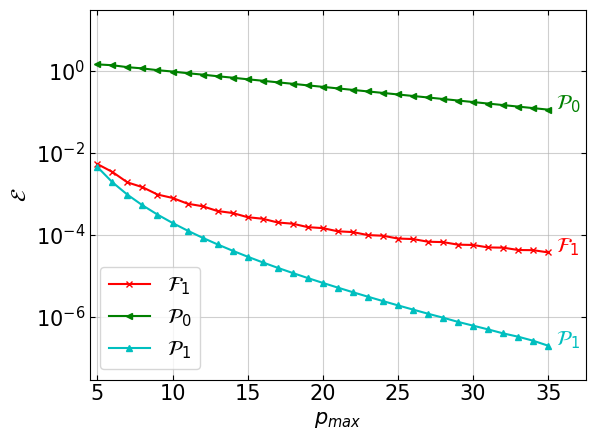
\includegraphics[width=.75\columnwidth]{plots/template_reconstruction_quadratic_sr.png}}\\
%\subfloat[Reconstructing the DBI Template]{\label{fig:b}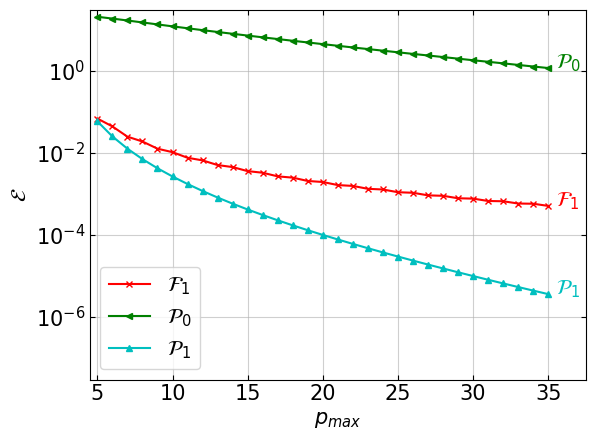
\includegraphics[width=.75\columnwidth]{plots/template_reconstruction_DBI.png}}
\subfloat[Reconstructing the Maldacena Template]{\label{fig:recon_a}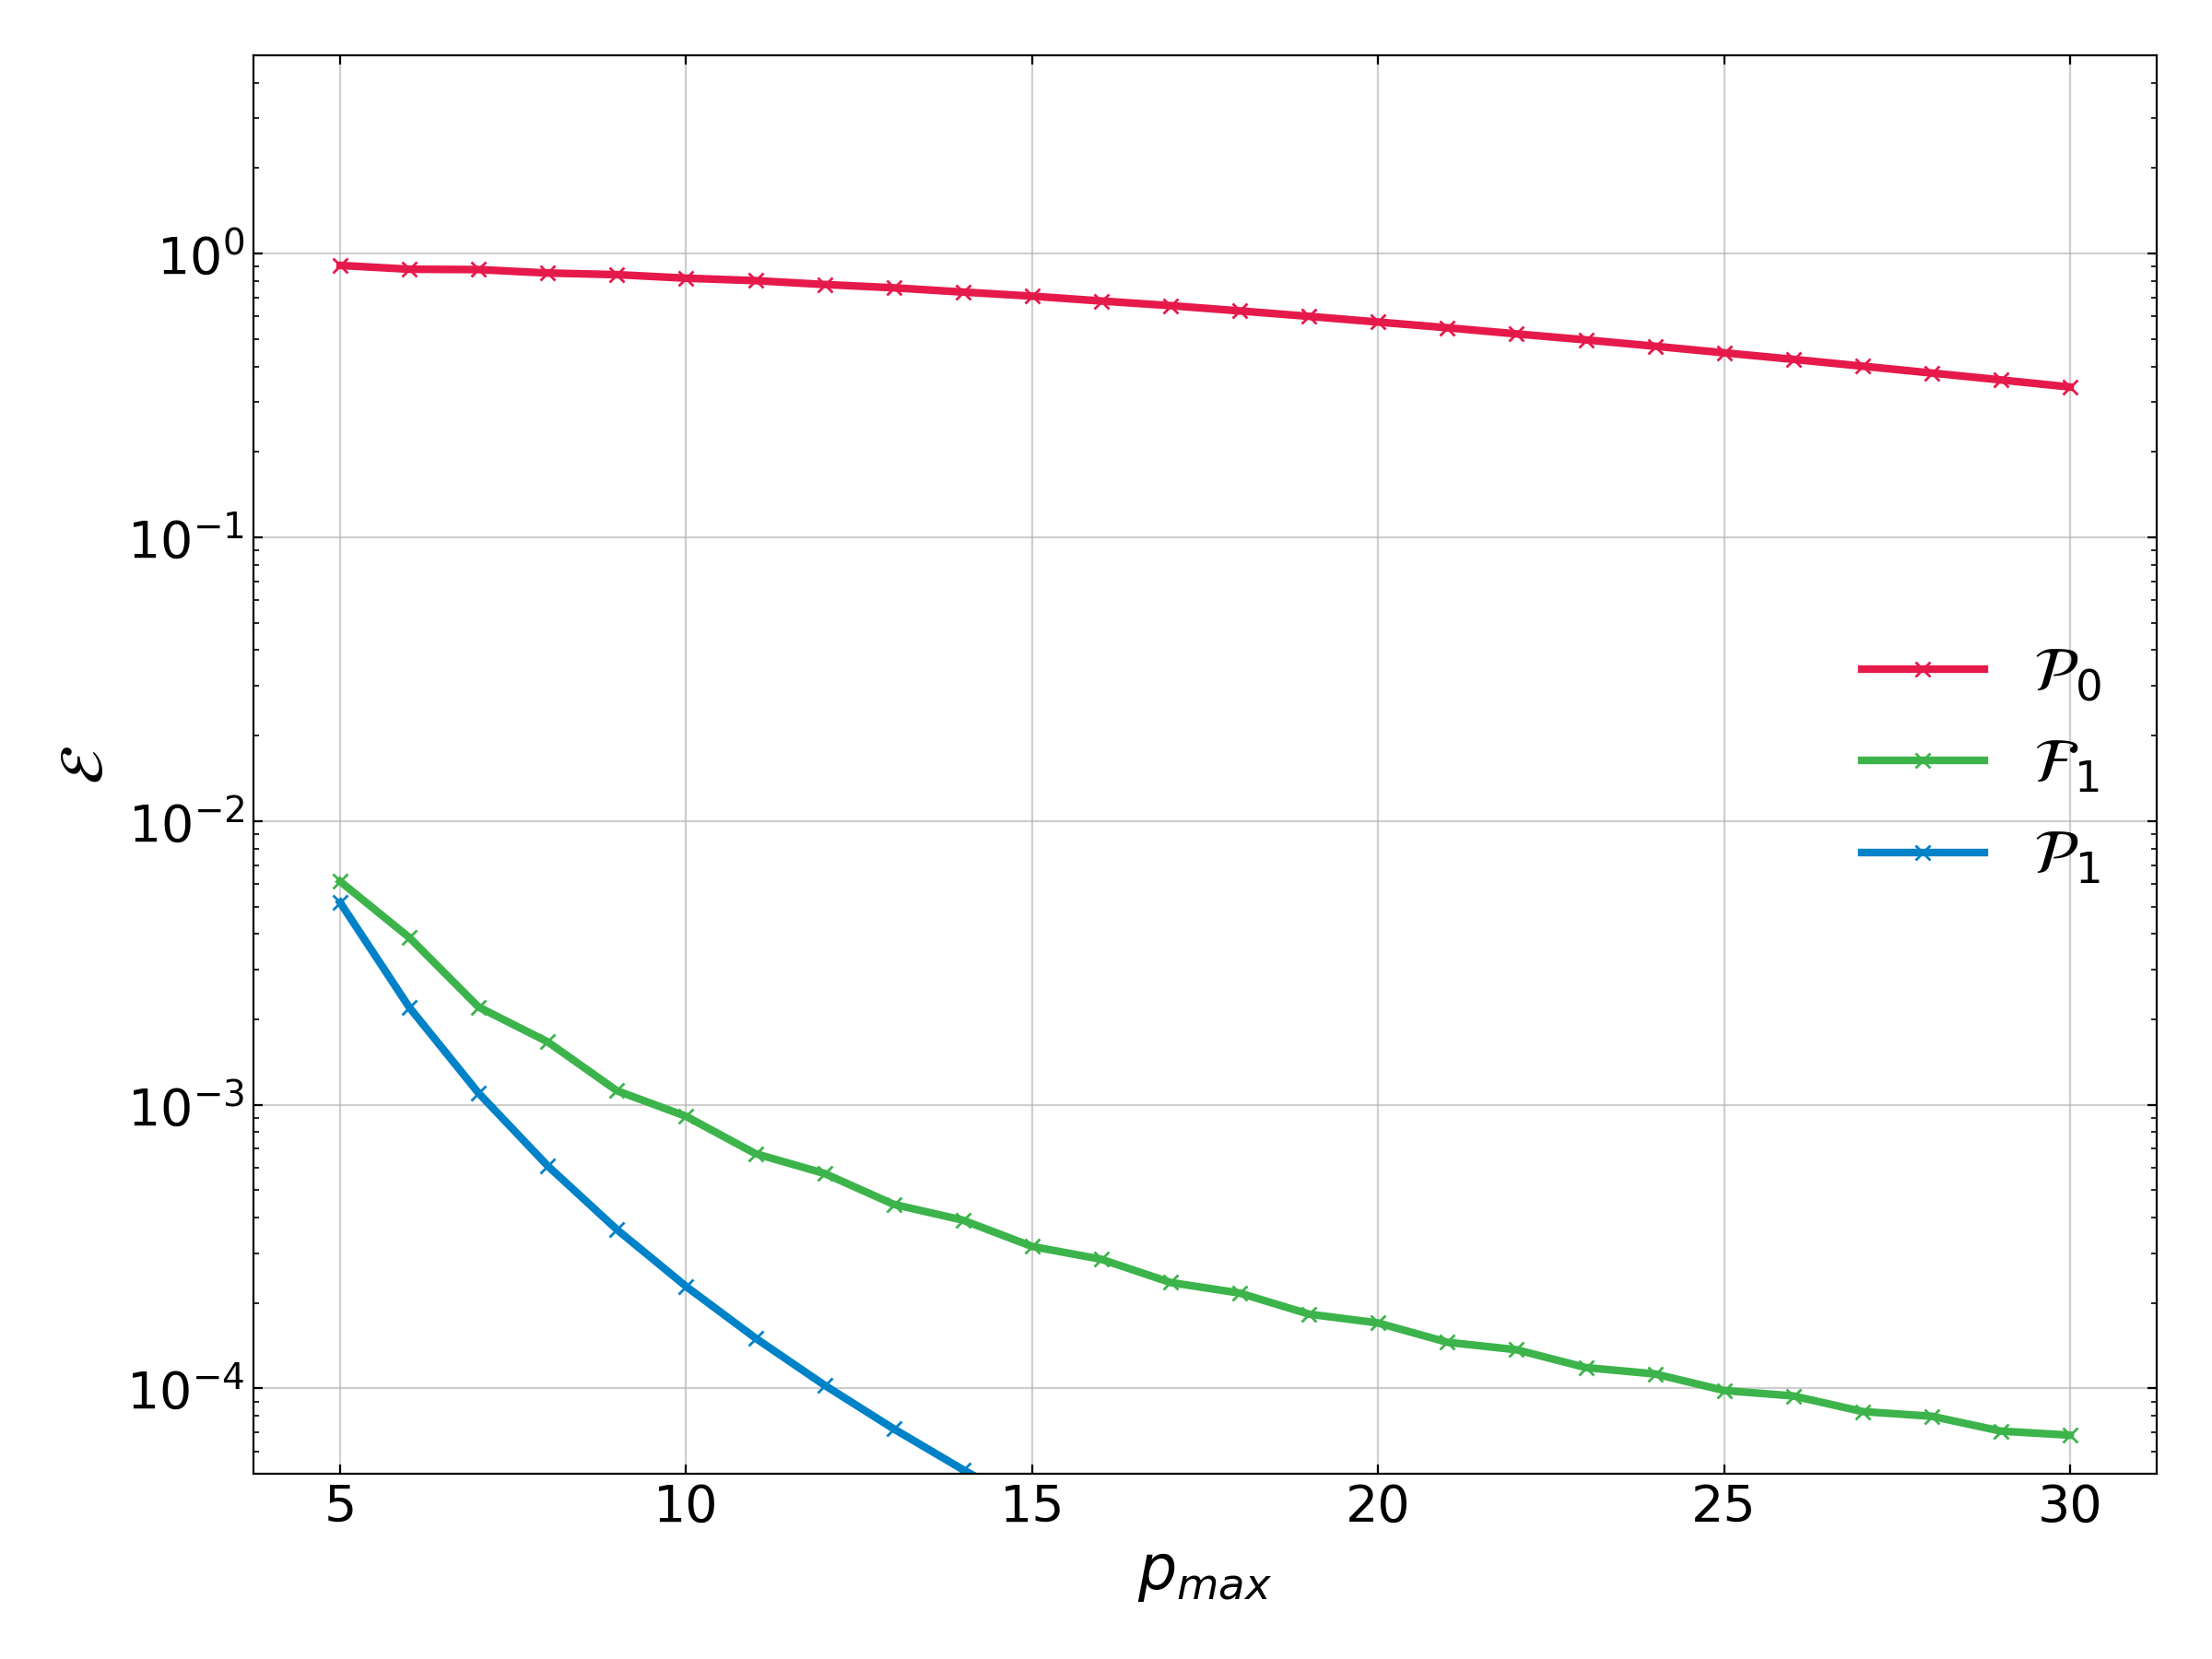
\includegraphics[width=.75\columnwidth]{pmax_reduction_plots_1_1000/malda.png}}\\
\subfloat[Reconstructing the DBI Template]{\label{fig:recon_b}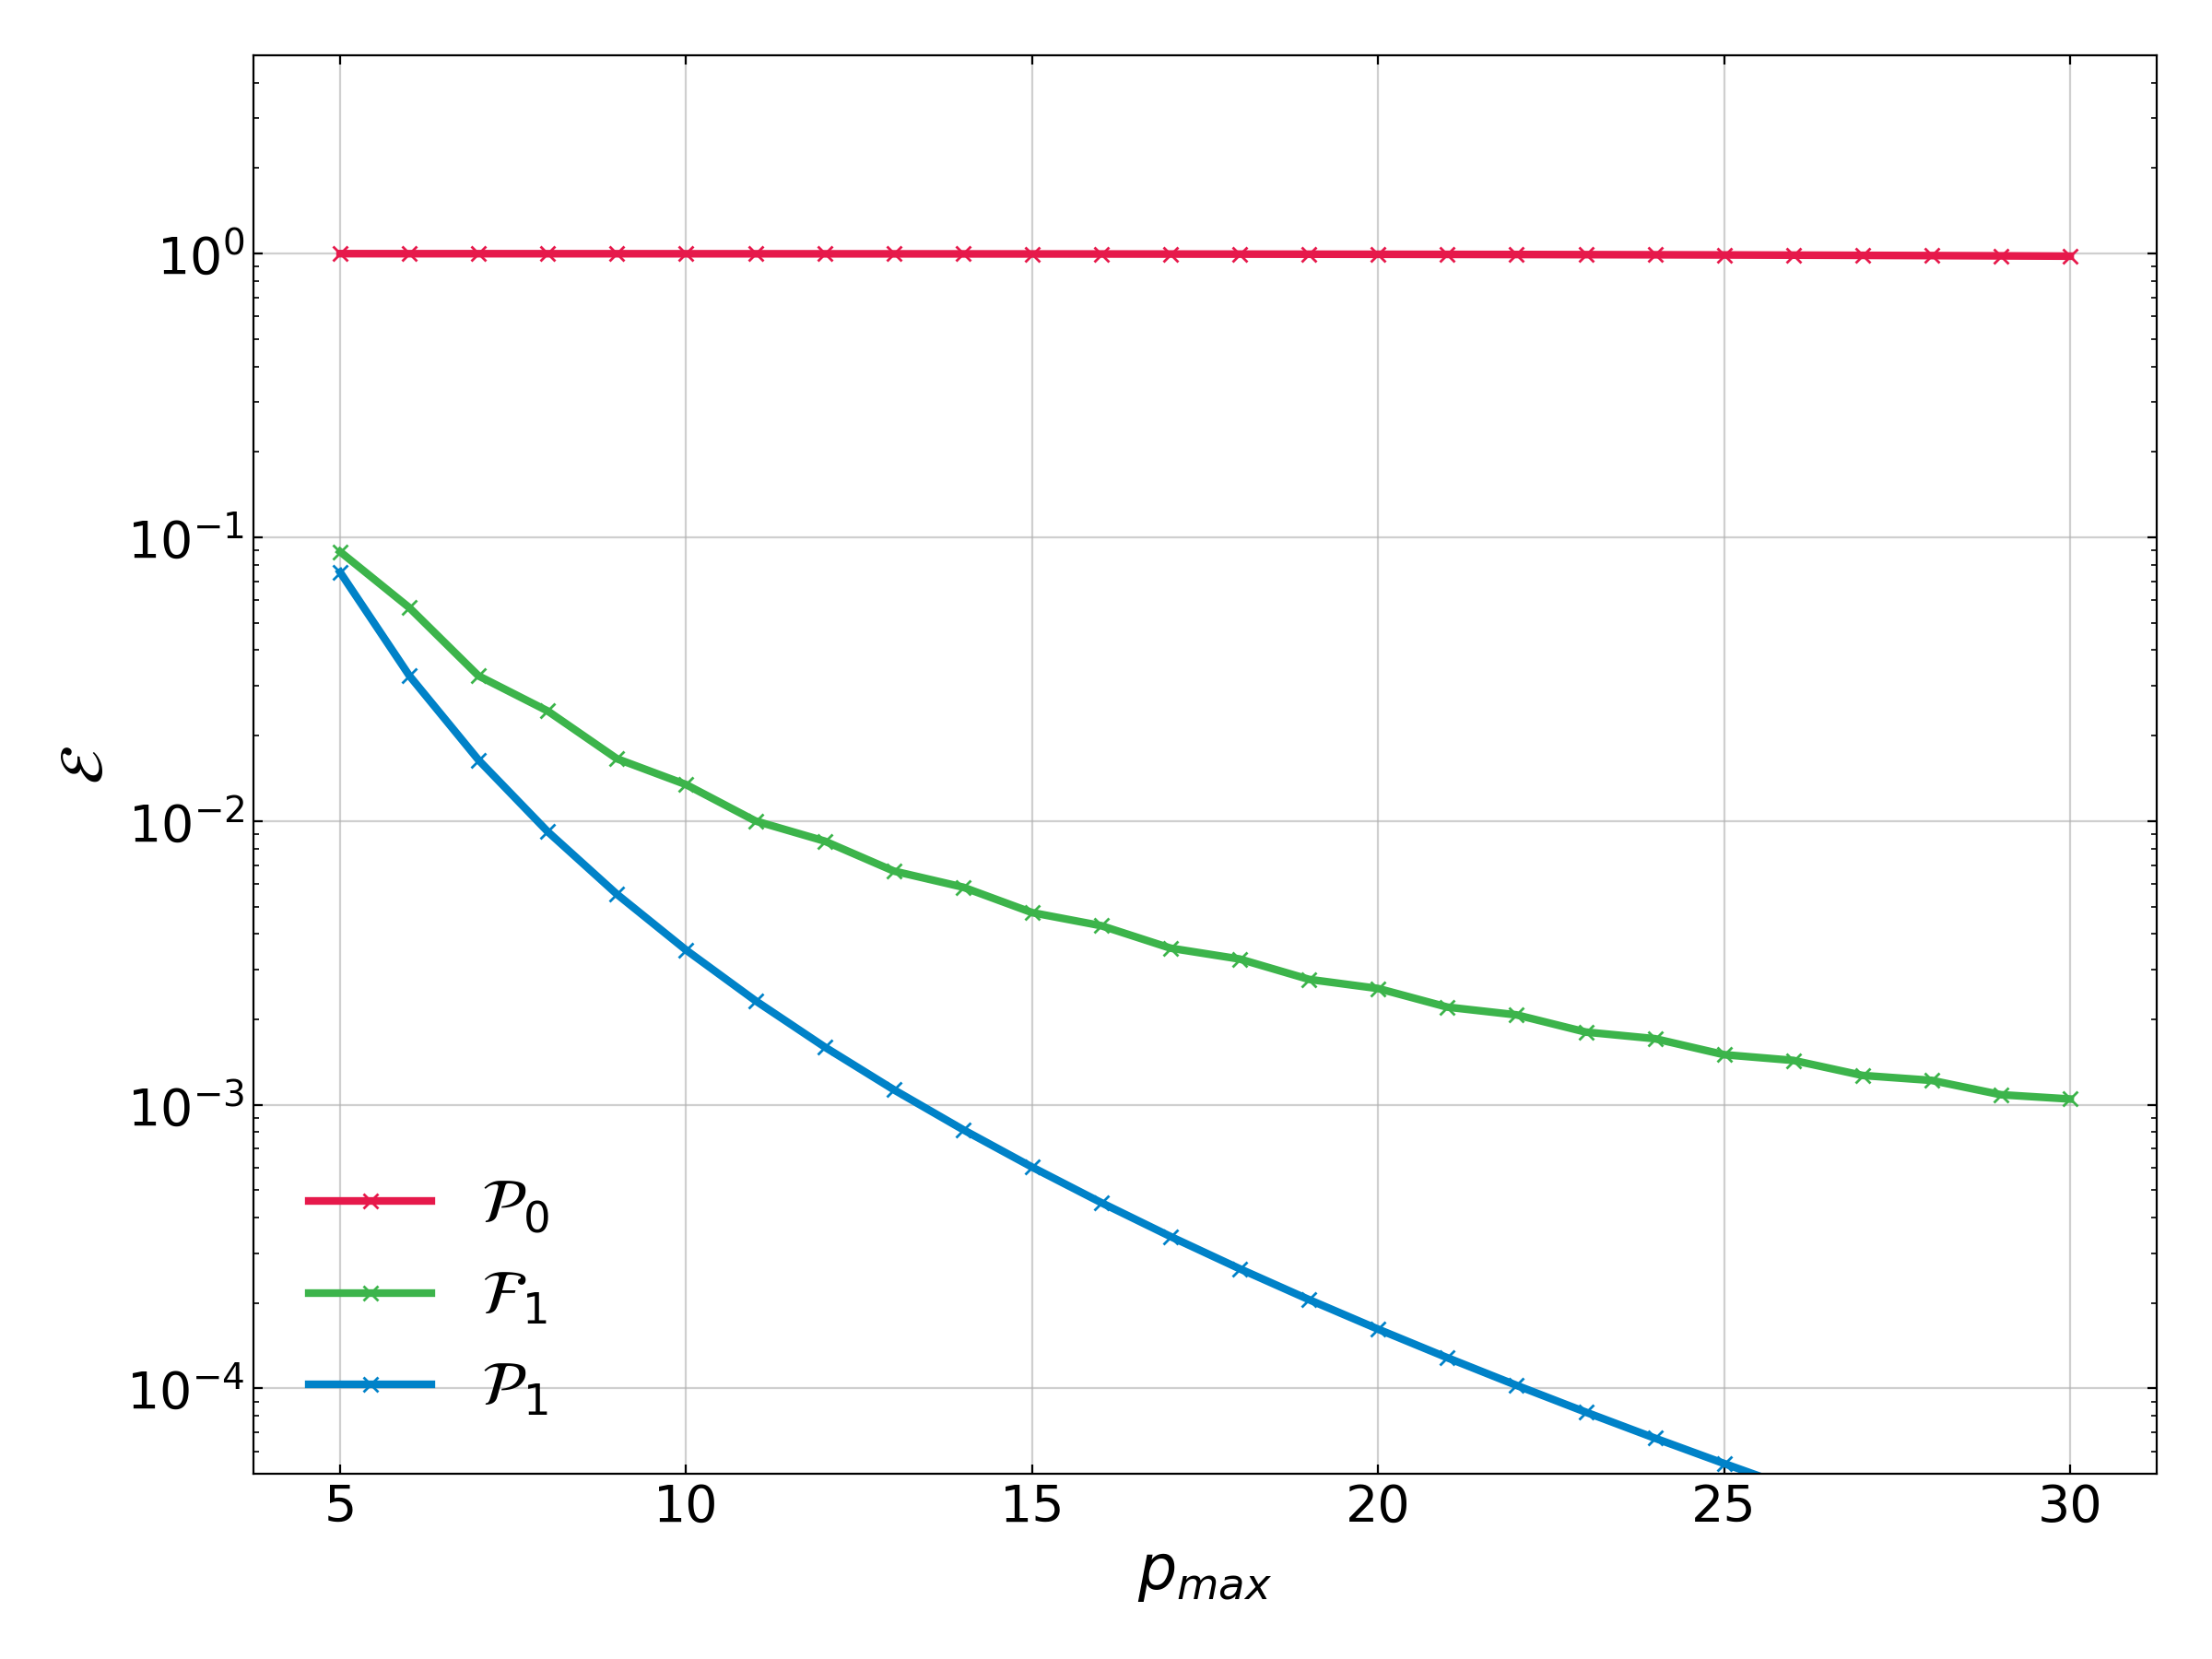
\includegraphics[width=.75\columnwidth]{pmax_reduction_plots_1_1000/dbi.png}}
\caption{
    Convergence comparisons for the Legendre and Fourier basis functions for (a) the Maldacena 
    template~\eqref{malda_shape} and (b) the DBI template~\eqref{dbi_shape}.
    The pure Legendre $\Lbasic$ basis requires many terms to fit the $1/k$ behaviour
    in both Maldacena's template~\eqref{malda_shape} and the DBI template~\eqref{dbi_shape}.
    In contrast, the $\Linvk$ basis (with an orthogonalised $1/k$ term) mitigates this dramatically, with the 
    error already reduced by a factor of $100$ at $\Pmax=5$.
    The Fourier $\Finvk$ basis performs well, but converges more slowly than the $\Linvk$ basis.
    Note that the convergence errors for~\eqref{dbi_shape} are larger than~\eqref{malda_shape} because of the larger contributions outside the tetrapyd dominating the fit.
    In this plot and the following, unless otherwise stated, $\kmax=1000\kmin$.
}\label{fig:recon_malda_dbi}
\end{figure}


Next, we investigate oscillatory model templates.
The simple feature model~\eqref{cos_shape} and the resonance model~\eqref{ln_cos_shape}
have scale dependence, but no shape dependence (in that they only depend on the perimeter
of the triangle, $K=k_1+k_2+k_3$).
We test our sets of basis functions on these two shapes,
and also when they are multiplied by~\eqref{dbi_shape} to obtain a feature
template with both shape and scale dependence.
As shown in figure~\ref{fig:recon_osc_dbiosc},
$\Fbasic$ naturally outperform the basis sets built from Legendre modes for a pure oscillation.
However when the equilateral-type DBI template~\eqref{dbi_shape} is superimposed, even the augmented Fourier modes
$\Finvk$ converge poorly. Instead, the basis sets built from Legendre modes offer a better more robust option,
with the $\scalingbasis$ basis performing best.
In figure~\ref{fig:log_recon_osc_dbiosc} we see that for a logarithmic
oscillation, the $\resobasis$ basis converges in the fewest modes.


\begin{figure}[!pth]
\centering     %%% not \center
%\subfloat[$\cos(f(k_1+k_2+k_3))$]{\label{fig:a}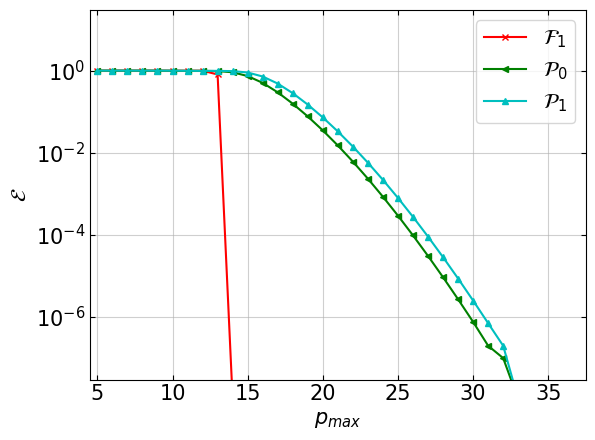
\includegraphics[width=.75\columnwidth]{plots/template_reconstruction_osc5.png}}\\
%\subfloat[$\cos(f(k_1+k_2+k_3))S^{DBI}$]{\label{fig:a}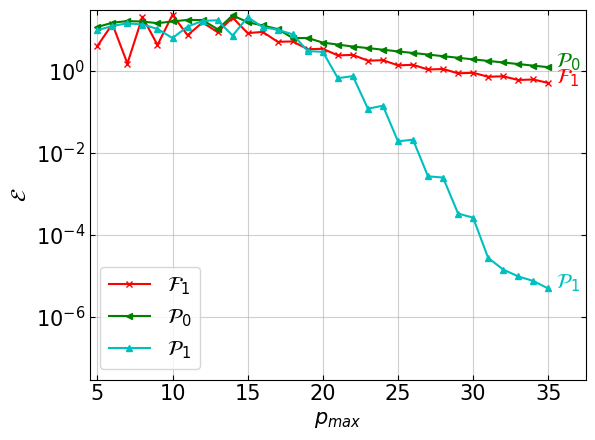
\includegraphics[width=.75\columnwidth]{plots/template_reconstruction_DBI_osc5.png}}
\subfloat[$\cos(f(k_1+k_2+k_3))$]{\label{fig:reduction_a}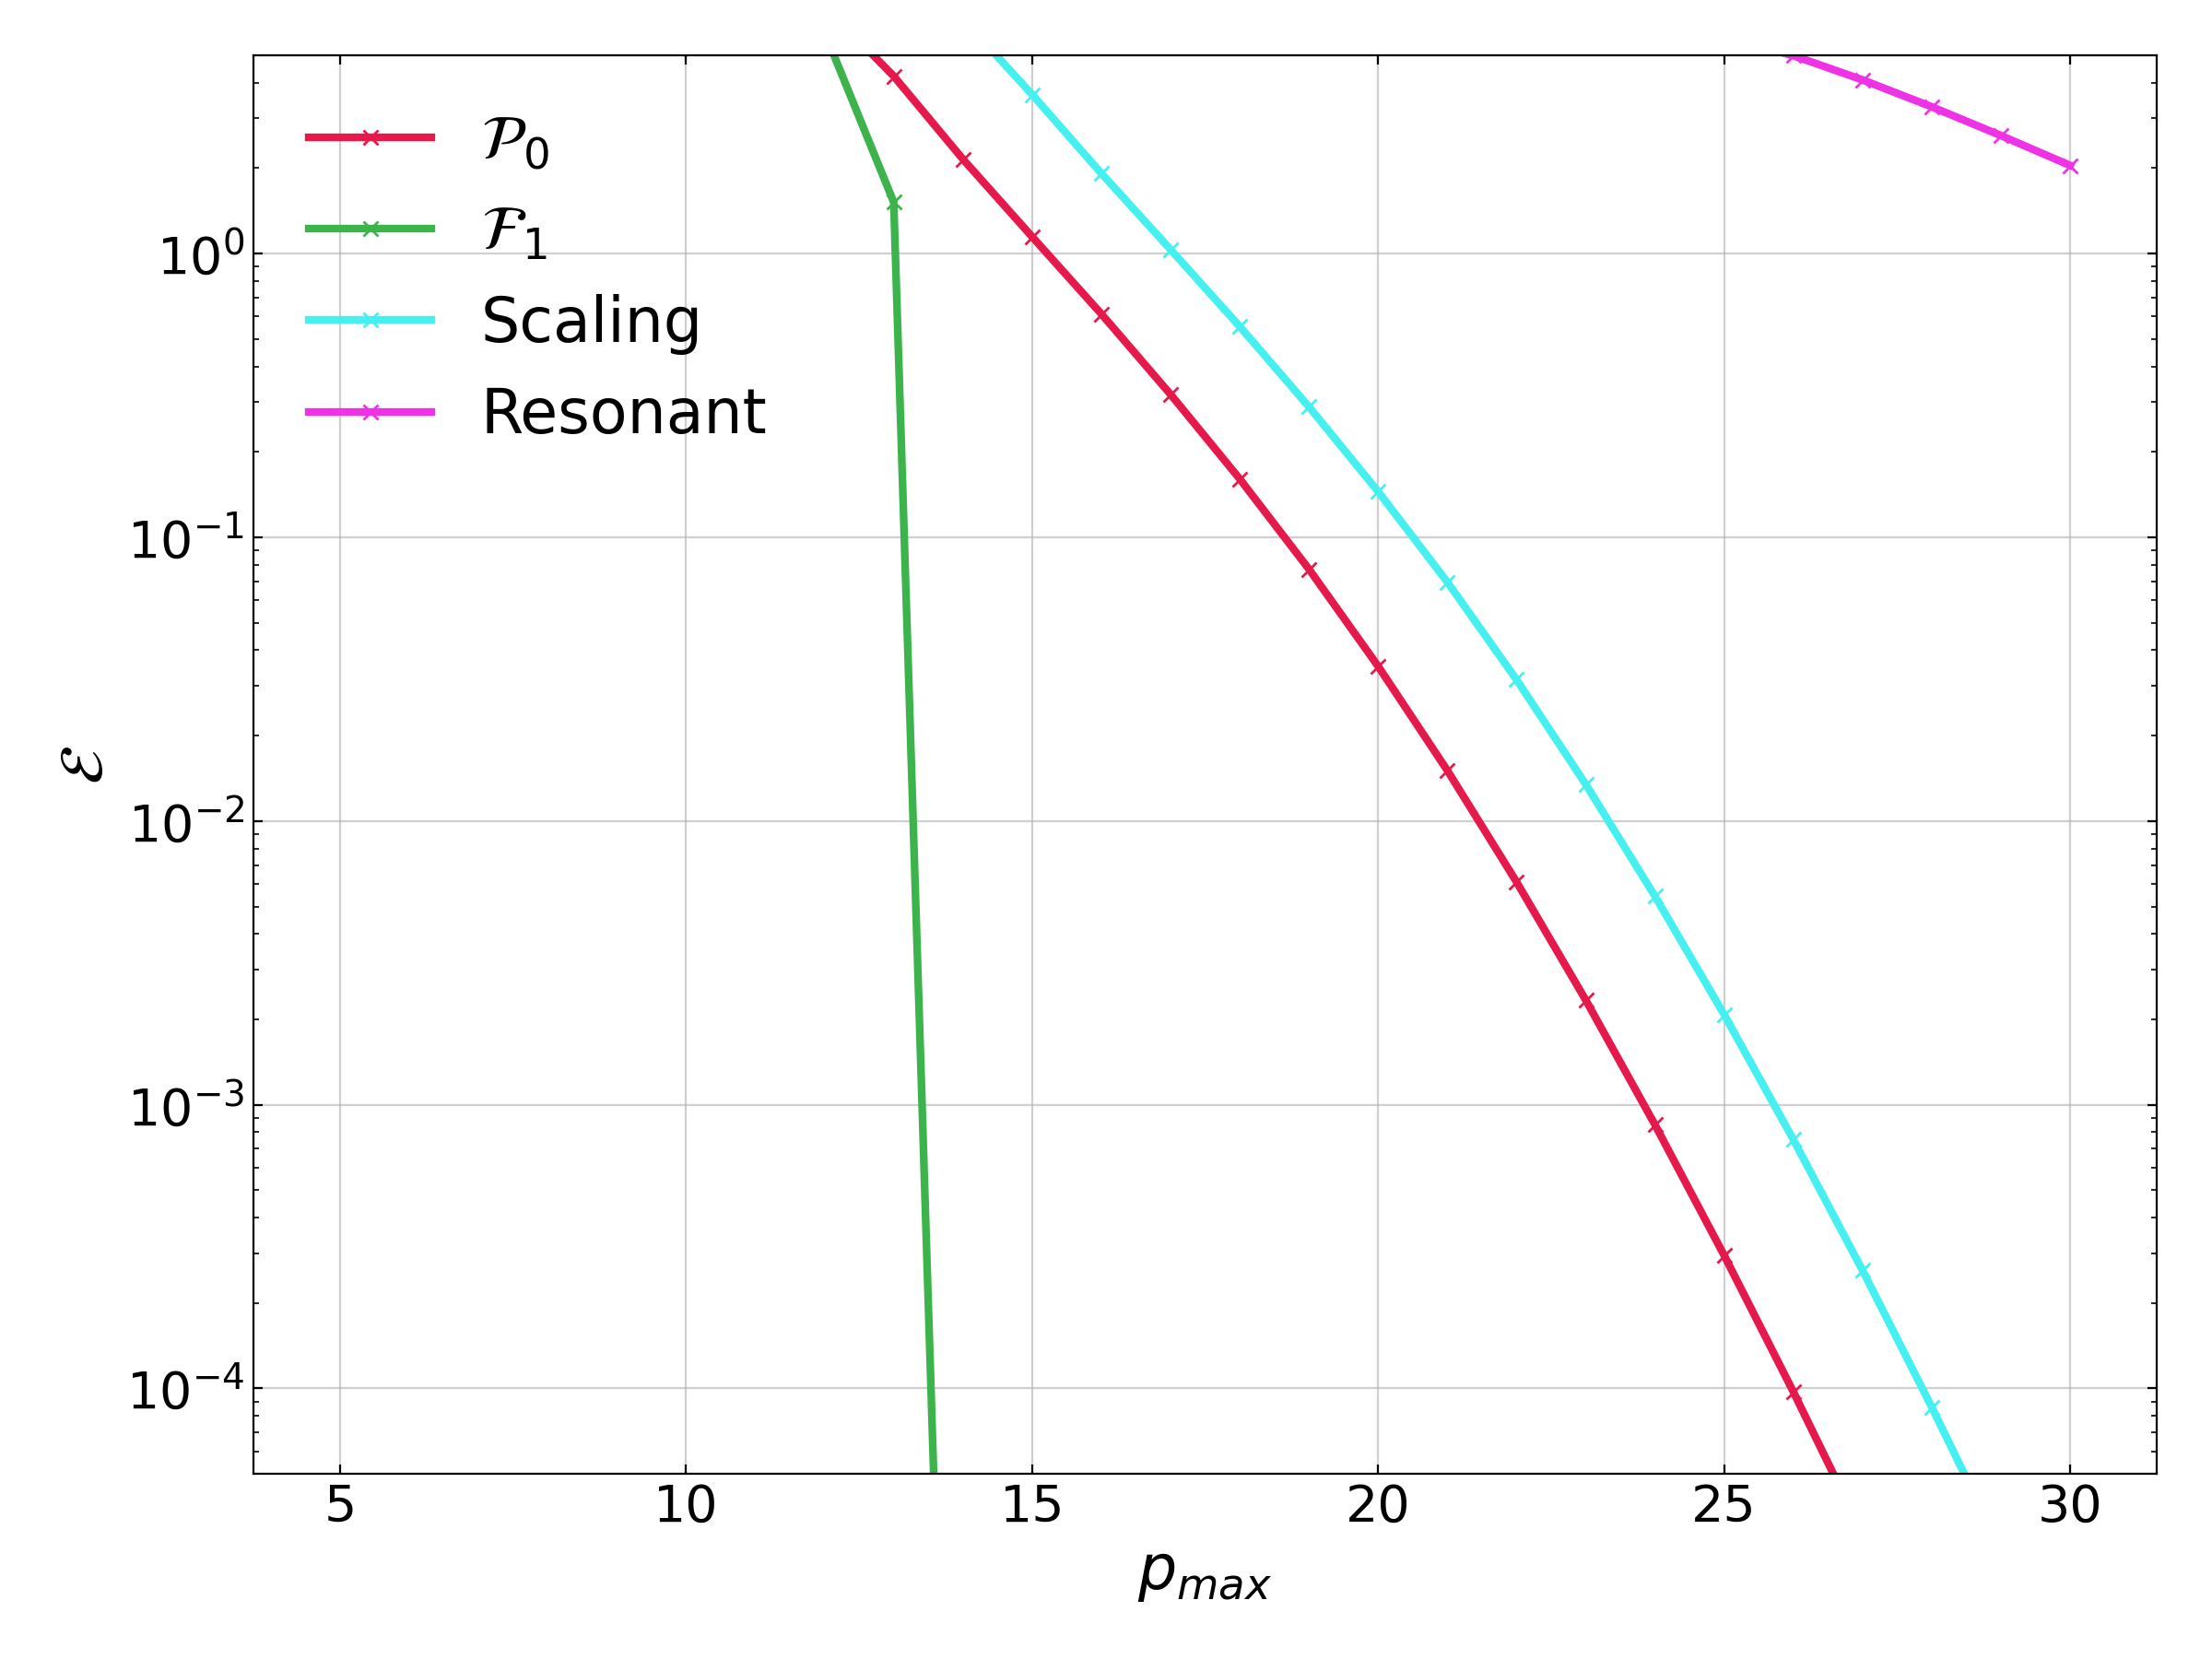
\includegraphics[width=.75\columnwidth]{pmax_reduction_plots_1_1000/cos15.png}}\\
\subfloat[$\cos(f(k_1+k_2+k_3))S^{DBI}$]{\label{fig:reduction_b}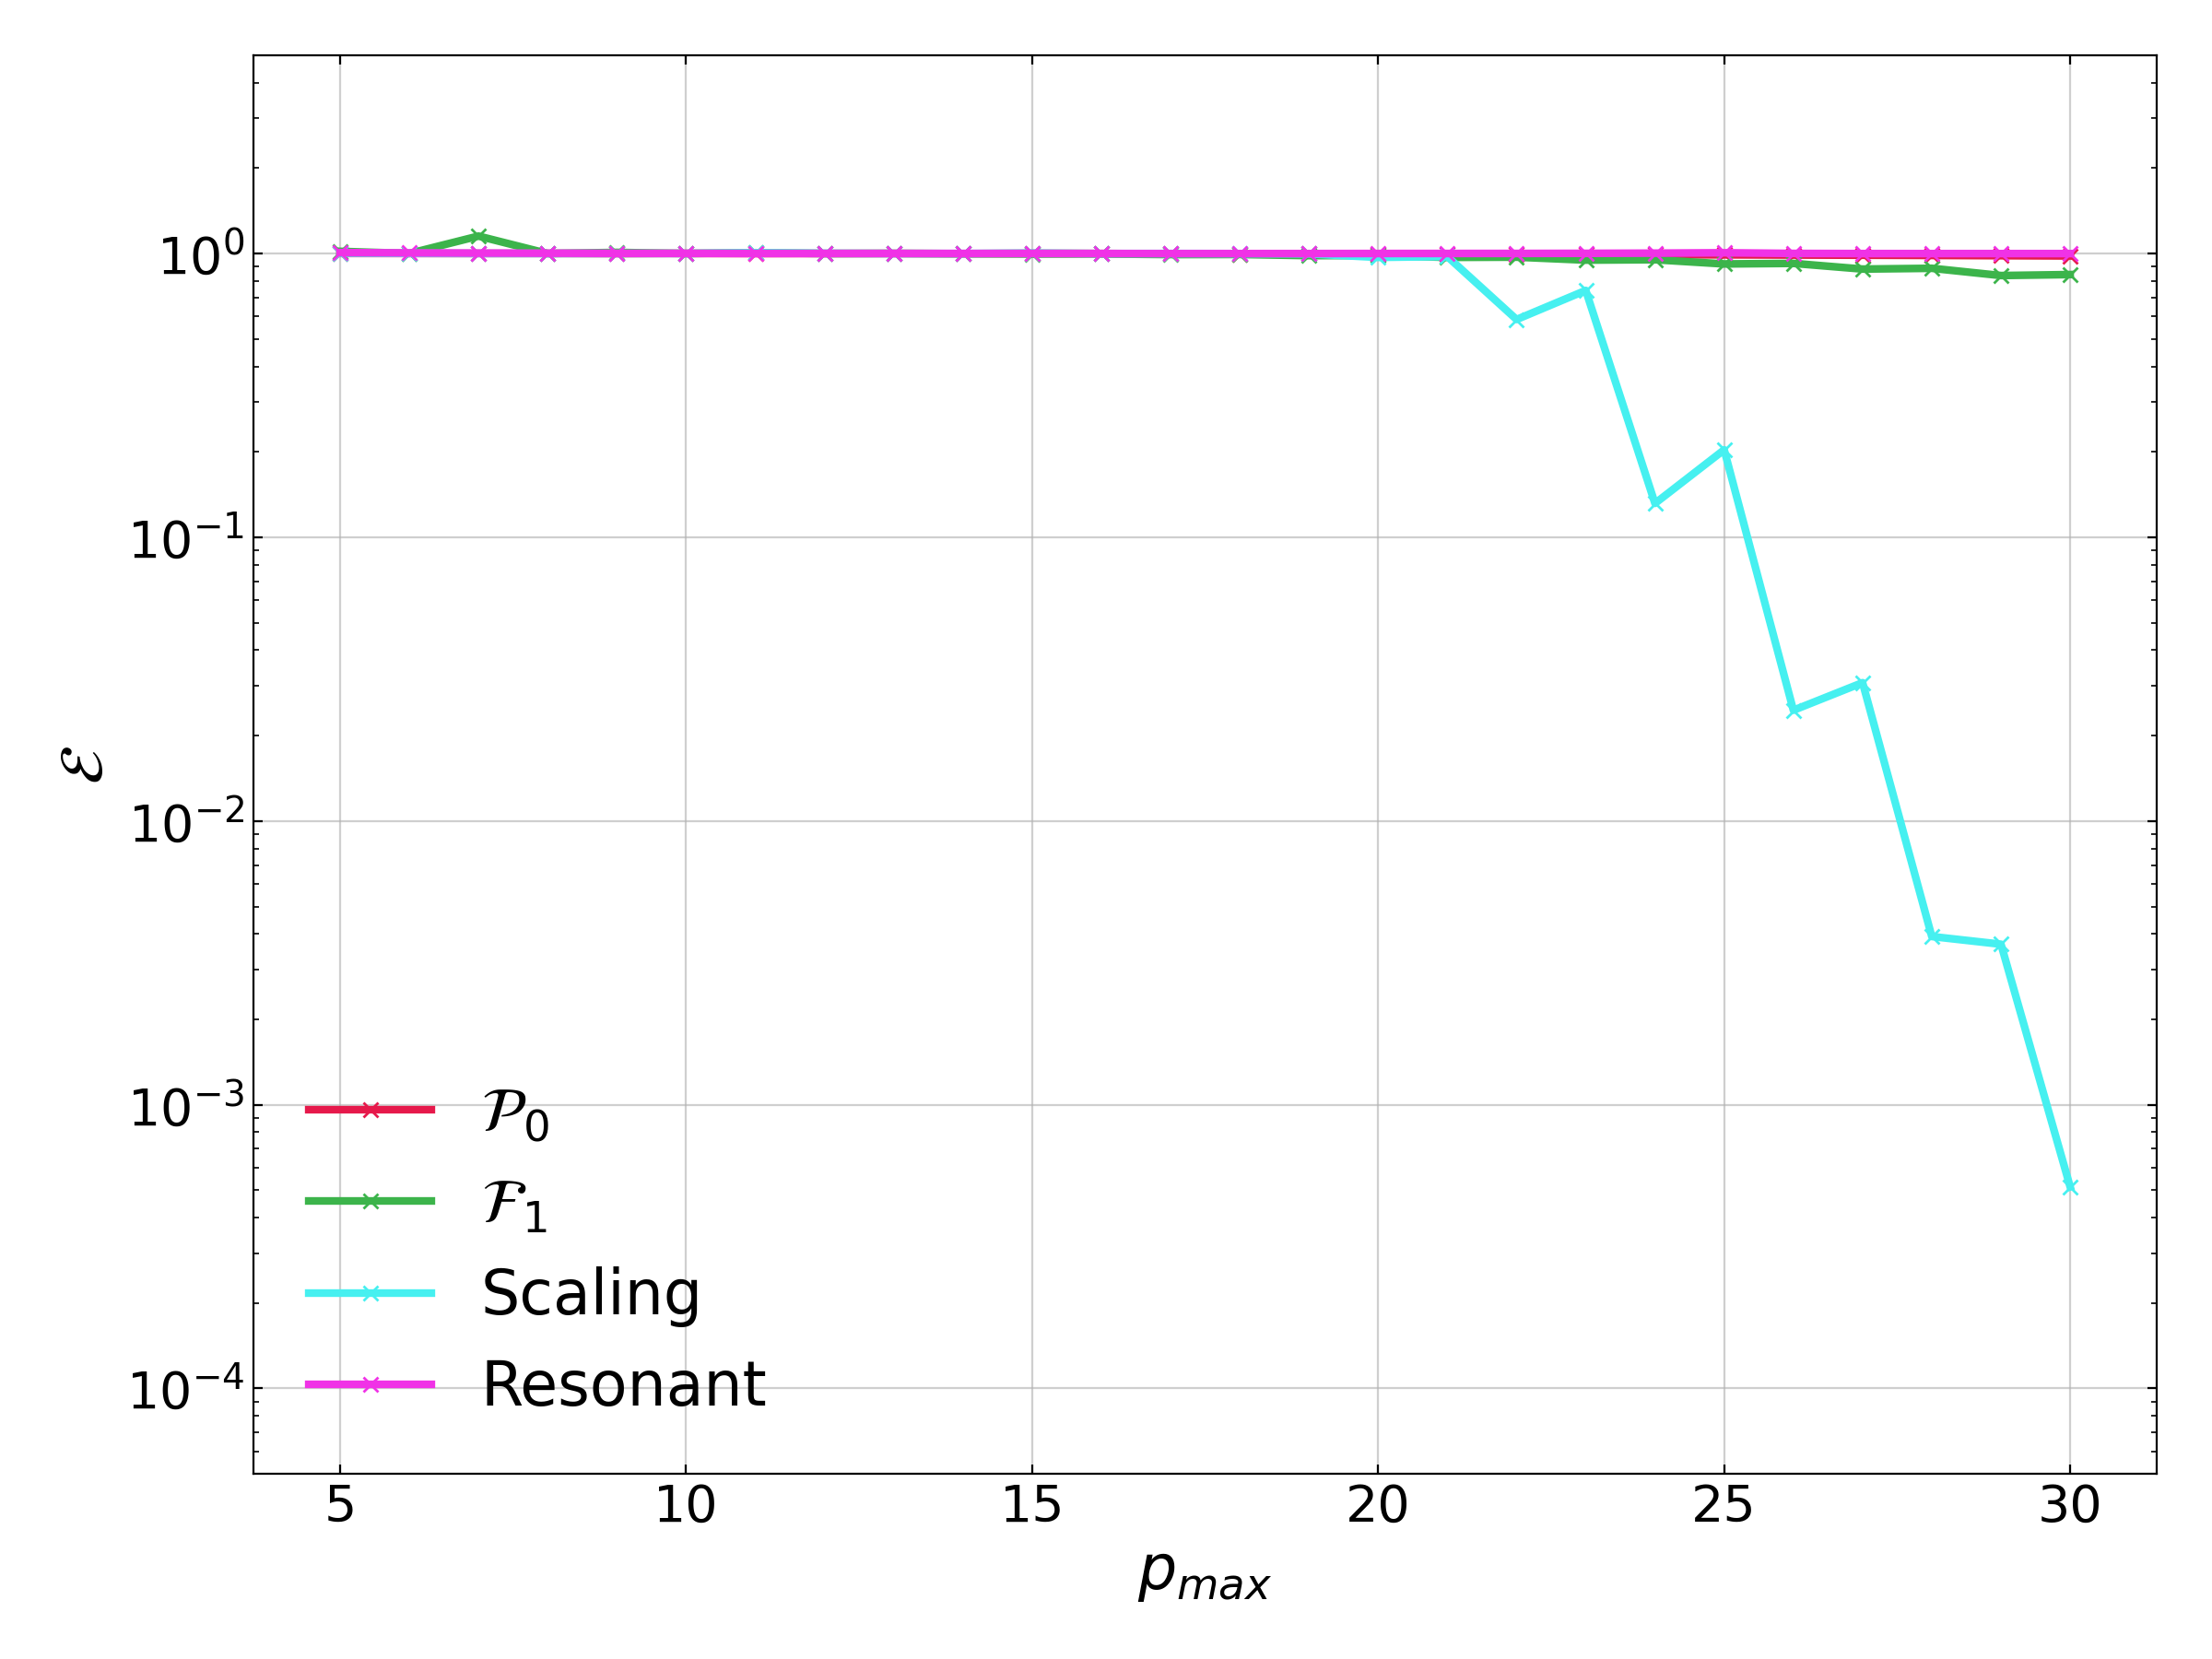
\includegraphics[width=.75\columnwidth]{pmax_reduction_plots_1_1000/dbi_cos15.png}}
\caption{
    Convergence comparison for oscillatory models.
    For linear oscillations we choose $f=150.64$ (so we obtain $15$ whole oscillations in the $k$-range).
    (a) As expected, the $\Finvk$ basis fits an oscillation with
    no shape dependence~\eqref{cos_shape} (that is periodic in the $k$-range) perfectly.
    For this special case, the $\Lbasic$, $\scalingbasis$ and $\resobasis$ sets of basis functions require more modes
    to accurately describe the shape. (b) However, moving to the more complex and realistic case of a
    feature with scale and shape dependence (in this case the product of~\eqref{dbi_shape}
    and~\eqref{cos_shape}), we see that again the $\scalingbasis$ basis converges with the fewest modes.
    Note that before the expansion has fully converged, the fit on the tetrapyd
    can actually degrade slightly when the basis set is extended. This is an artifact
    of fitting on the cube and restricting~\eqref{relative_difference}
    to the physical configurations on the tetrapyd; when considered over the
    entire cube the fit improves monotonically.
    The $\resobasis$ basis, naturally, does not converge well to a linear oscillation.
}\label{fig:recon_osc_dbiosc}
\end{figure}
\begin{figure}[!pth]
\centering     %%% not \center
%\subfloat[$\cos(f\log(k_1+k_2+k_3))$]{\label{fig:a}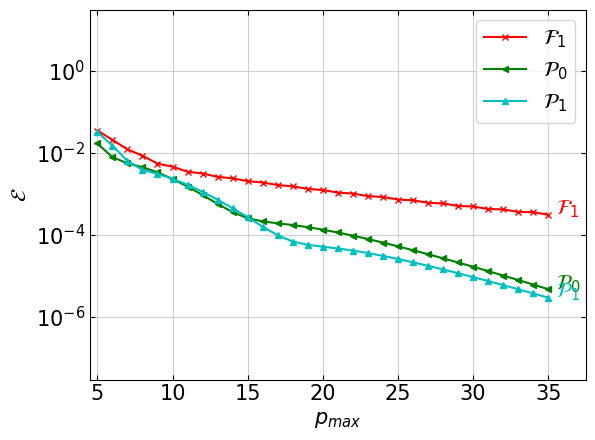
\includegraphics[width=.75\columnwidth]{plots/template_reconstruction_logosc2.png}}\\
%\subfloat[$\cos(f\log(k_1+k_2+k_3))S^{DBI}$]{\label{fig:a}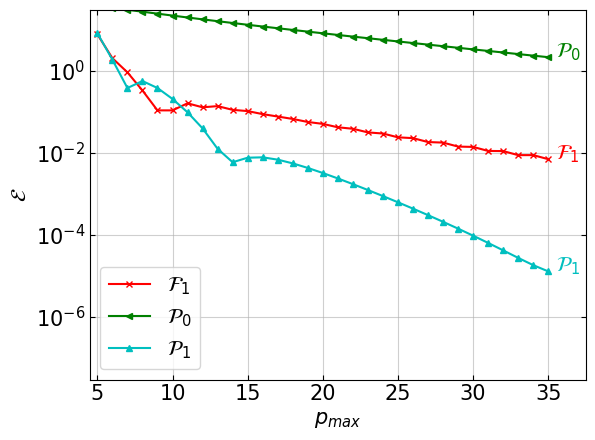
\includegraphics[width=.75\columnwidth]{plots/template_reconstruction_DBI_logosc2.png}}
\subfloat[$\cos(f\log(k_1+k_2+k_3))S^{DBI}$ on the tetrapyd]{\label{fig:reduction_c}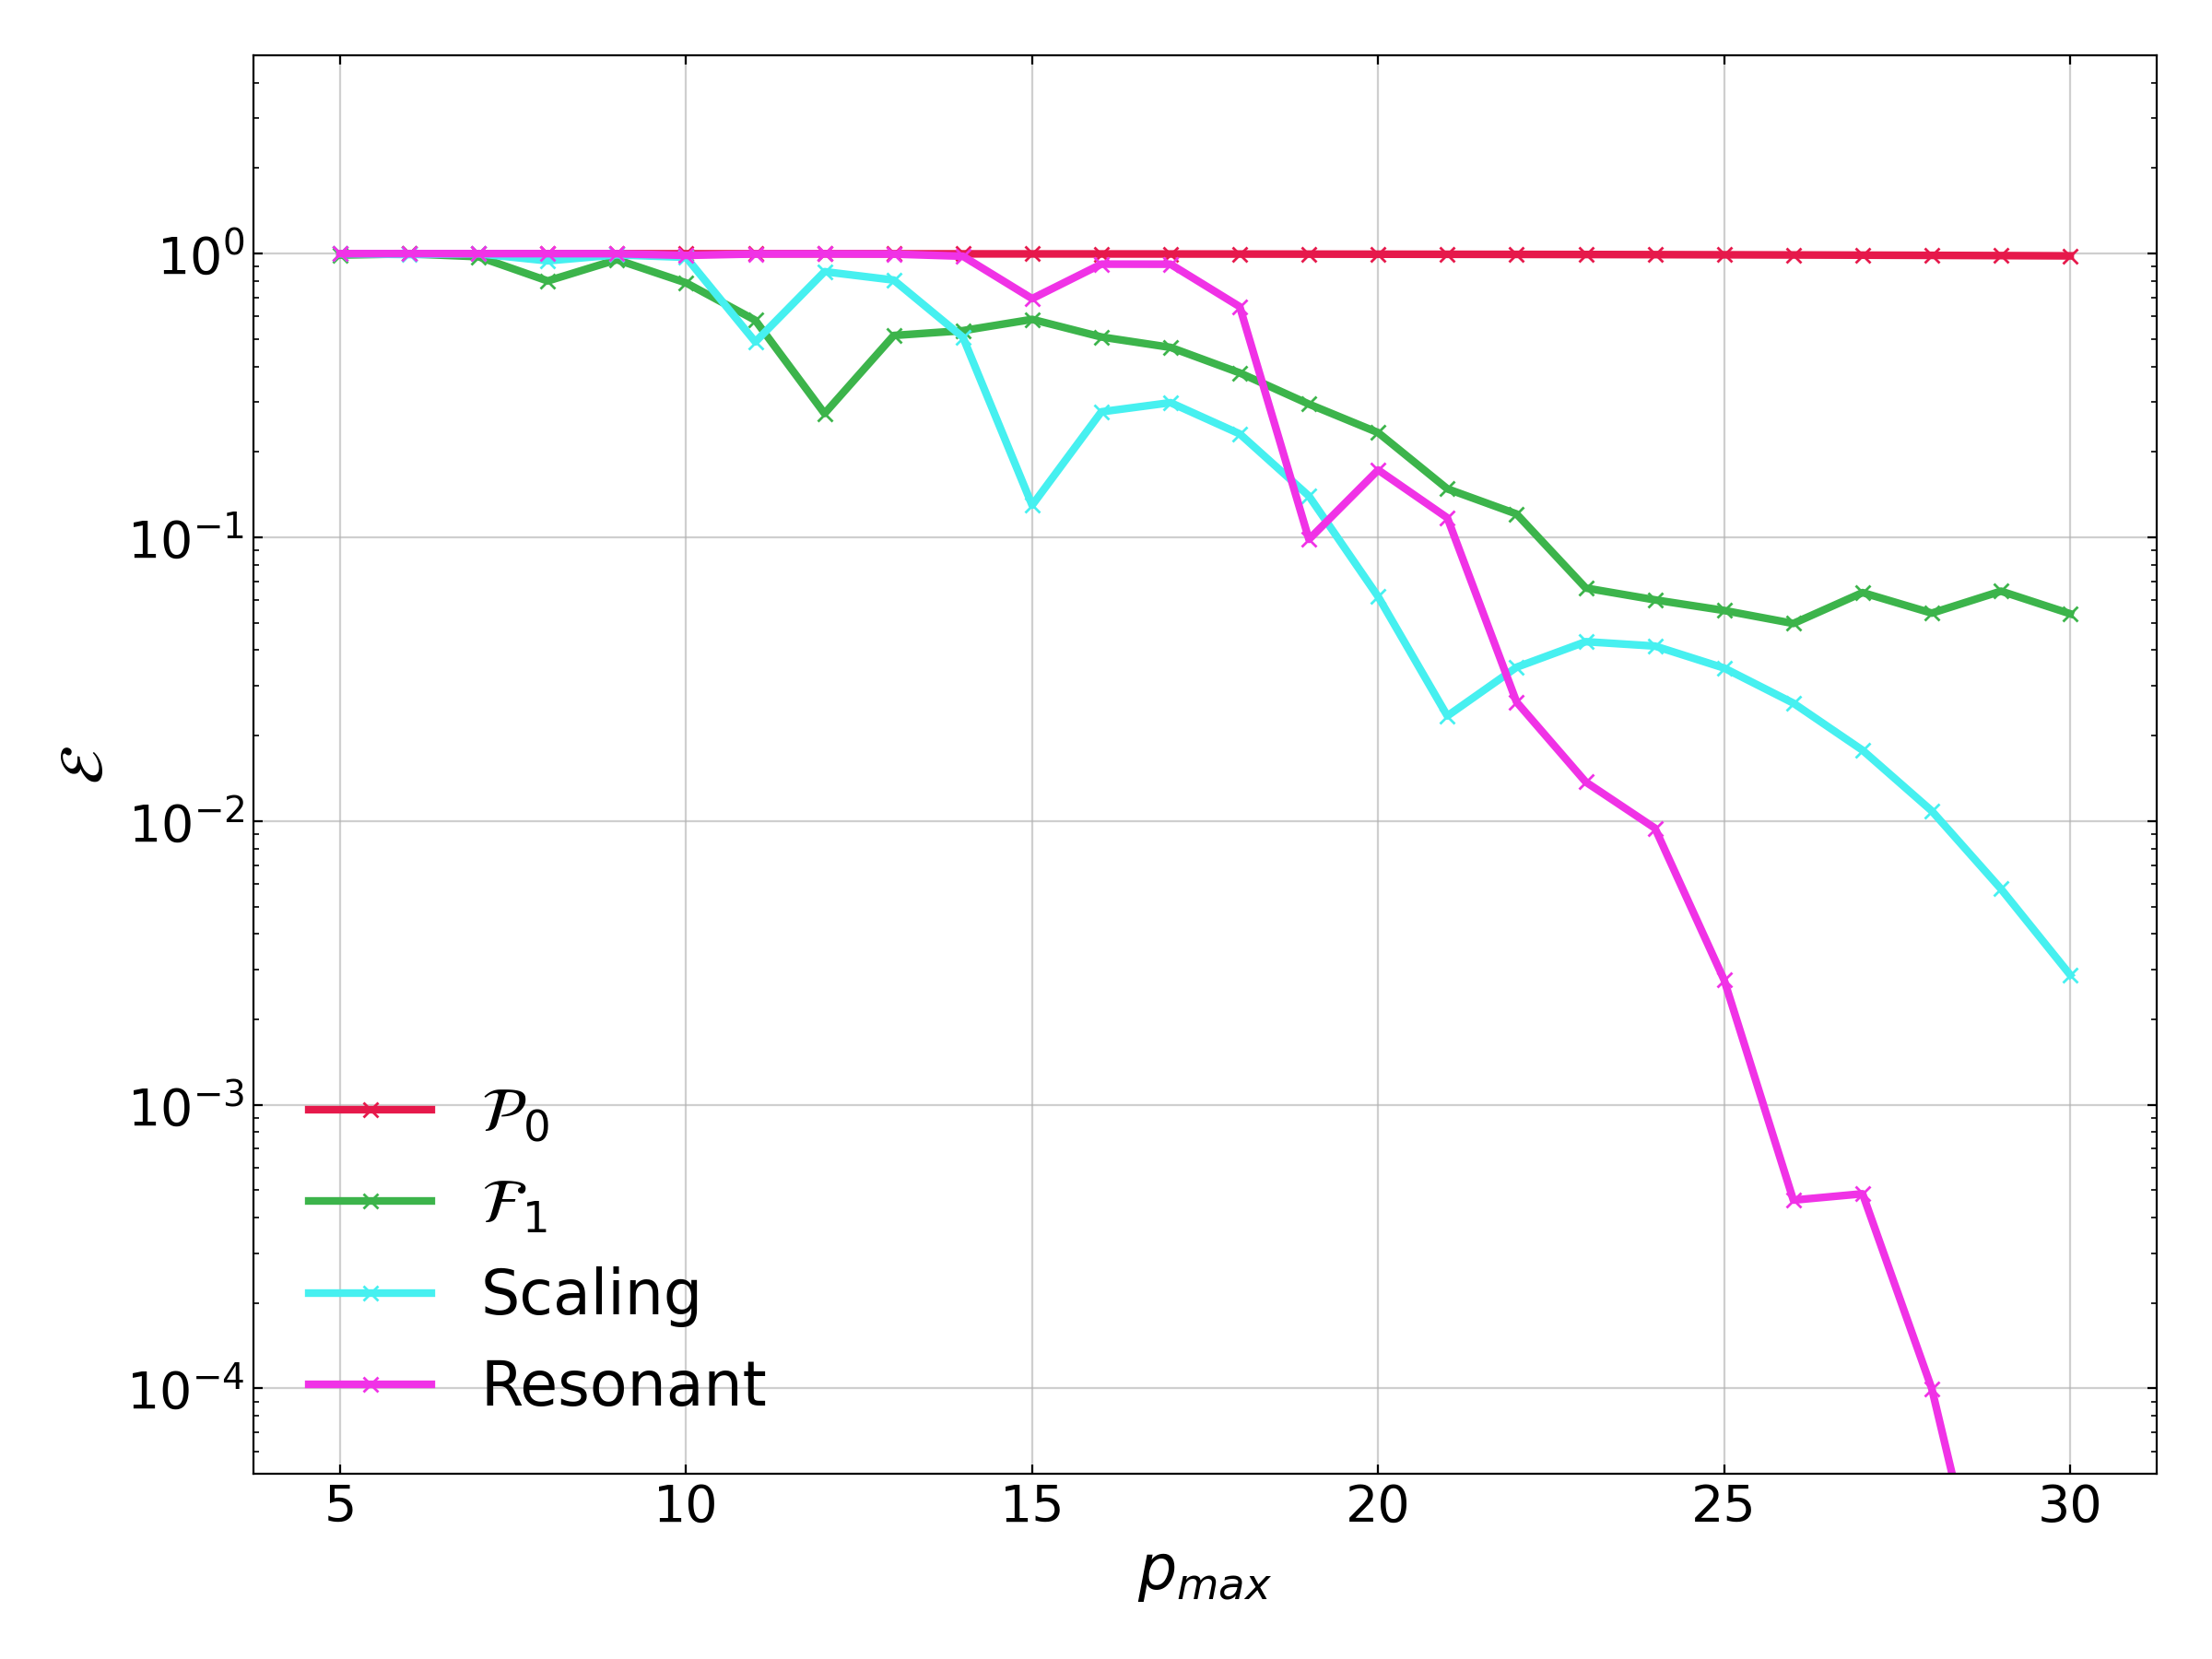
\includegraphics[width=.75\columnwidth]{pmax_reduction_plots_1_1000/dbi_cos5_log.png}}\\
\subfloat[$\cos(f\log(k_1+k_2+k_3))S^{DBI}$ on the cube]{\label{fig:reduction_ca}\includegraphics[width=.75\columnwidth]{pmax_cube_reduction_plots_1_1000/dbi_cos5_log_cube.png}}
\caption{
    %(a) The convergence for a log oscillation model~\eqref{ln_cos_shape} with no shape dependence.
    %For this type of feature, the $\Lbasic$ and $\Linvk$ sets of basis functions require fewer modes
    %to accurately describe the shape than the $\Finvk$ basis.
    %(b)
    %For the more complex and realistic case of a
    We plot the convergence of various basis sets for the more complex case of a resonant
    feature with scale and shape dependence, in this case the product of~\eqref{dbi_shape}
    and~\eqref{ln_cos_shape}.
    We choose $f=4.55$ (so we obtain $5$ whole oscillations in the $k$-range).
    (a) On the tetrapyd, we see that the $\scalingbasis$ basis struggles to converge for this fixed-frequency
    template, due to the combination of the high frequency logarithmic oscillation
    and the non-trivial shape dependence coming from $S^{DBI}(k_1,k_2,k_3)$.
    As expected for logarithmic oscillations,
    the $\resobasis$ basis performs best for this template, confirming that
    the basis functions defined in~\eqref{reso_basis_definition} perform well
    even when there is non-trivial shape dependence.
    (b) On the cube, we see that the results converge orders of magnitude faster---see
    discussion in section~\ref{sec:large_non_physical}.
}\label{fig:log_recon_osc_dbiosc}
\end{figure}

\begin{figure}[!pth]
\centering
%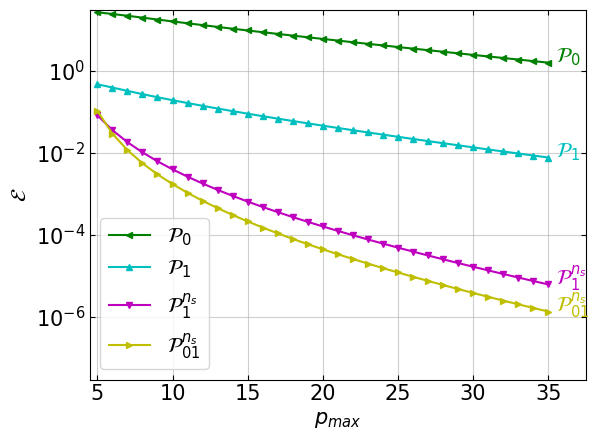
\includegraphics[width=0.8\columnwidth]{plots/template_reconstruction_DBI_ns.png}
%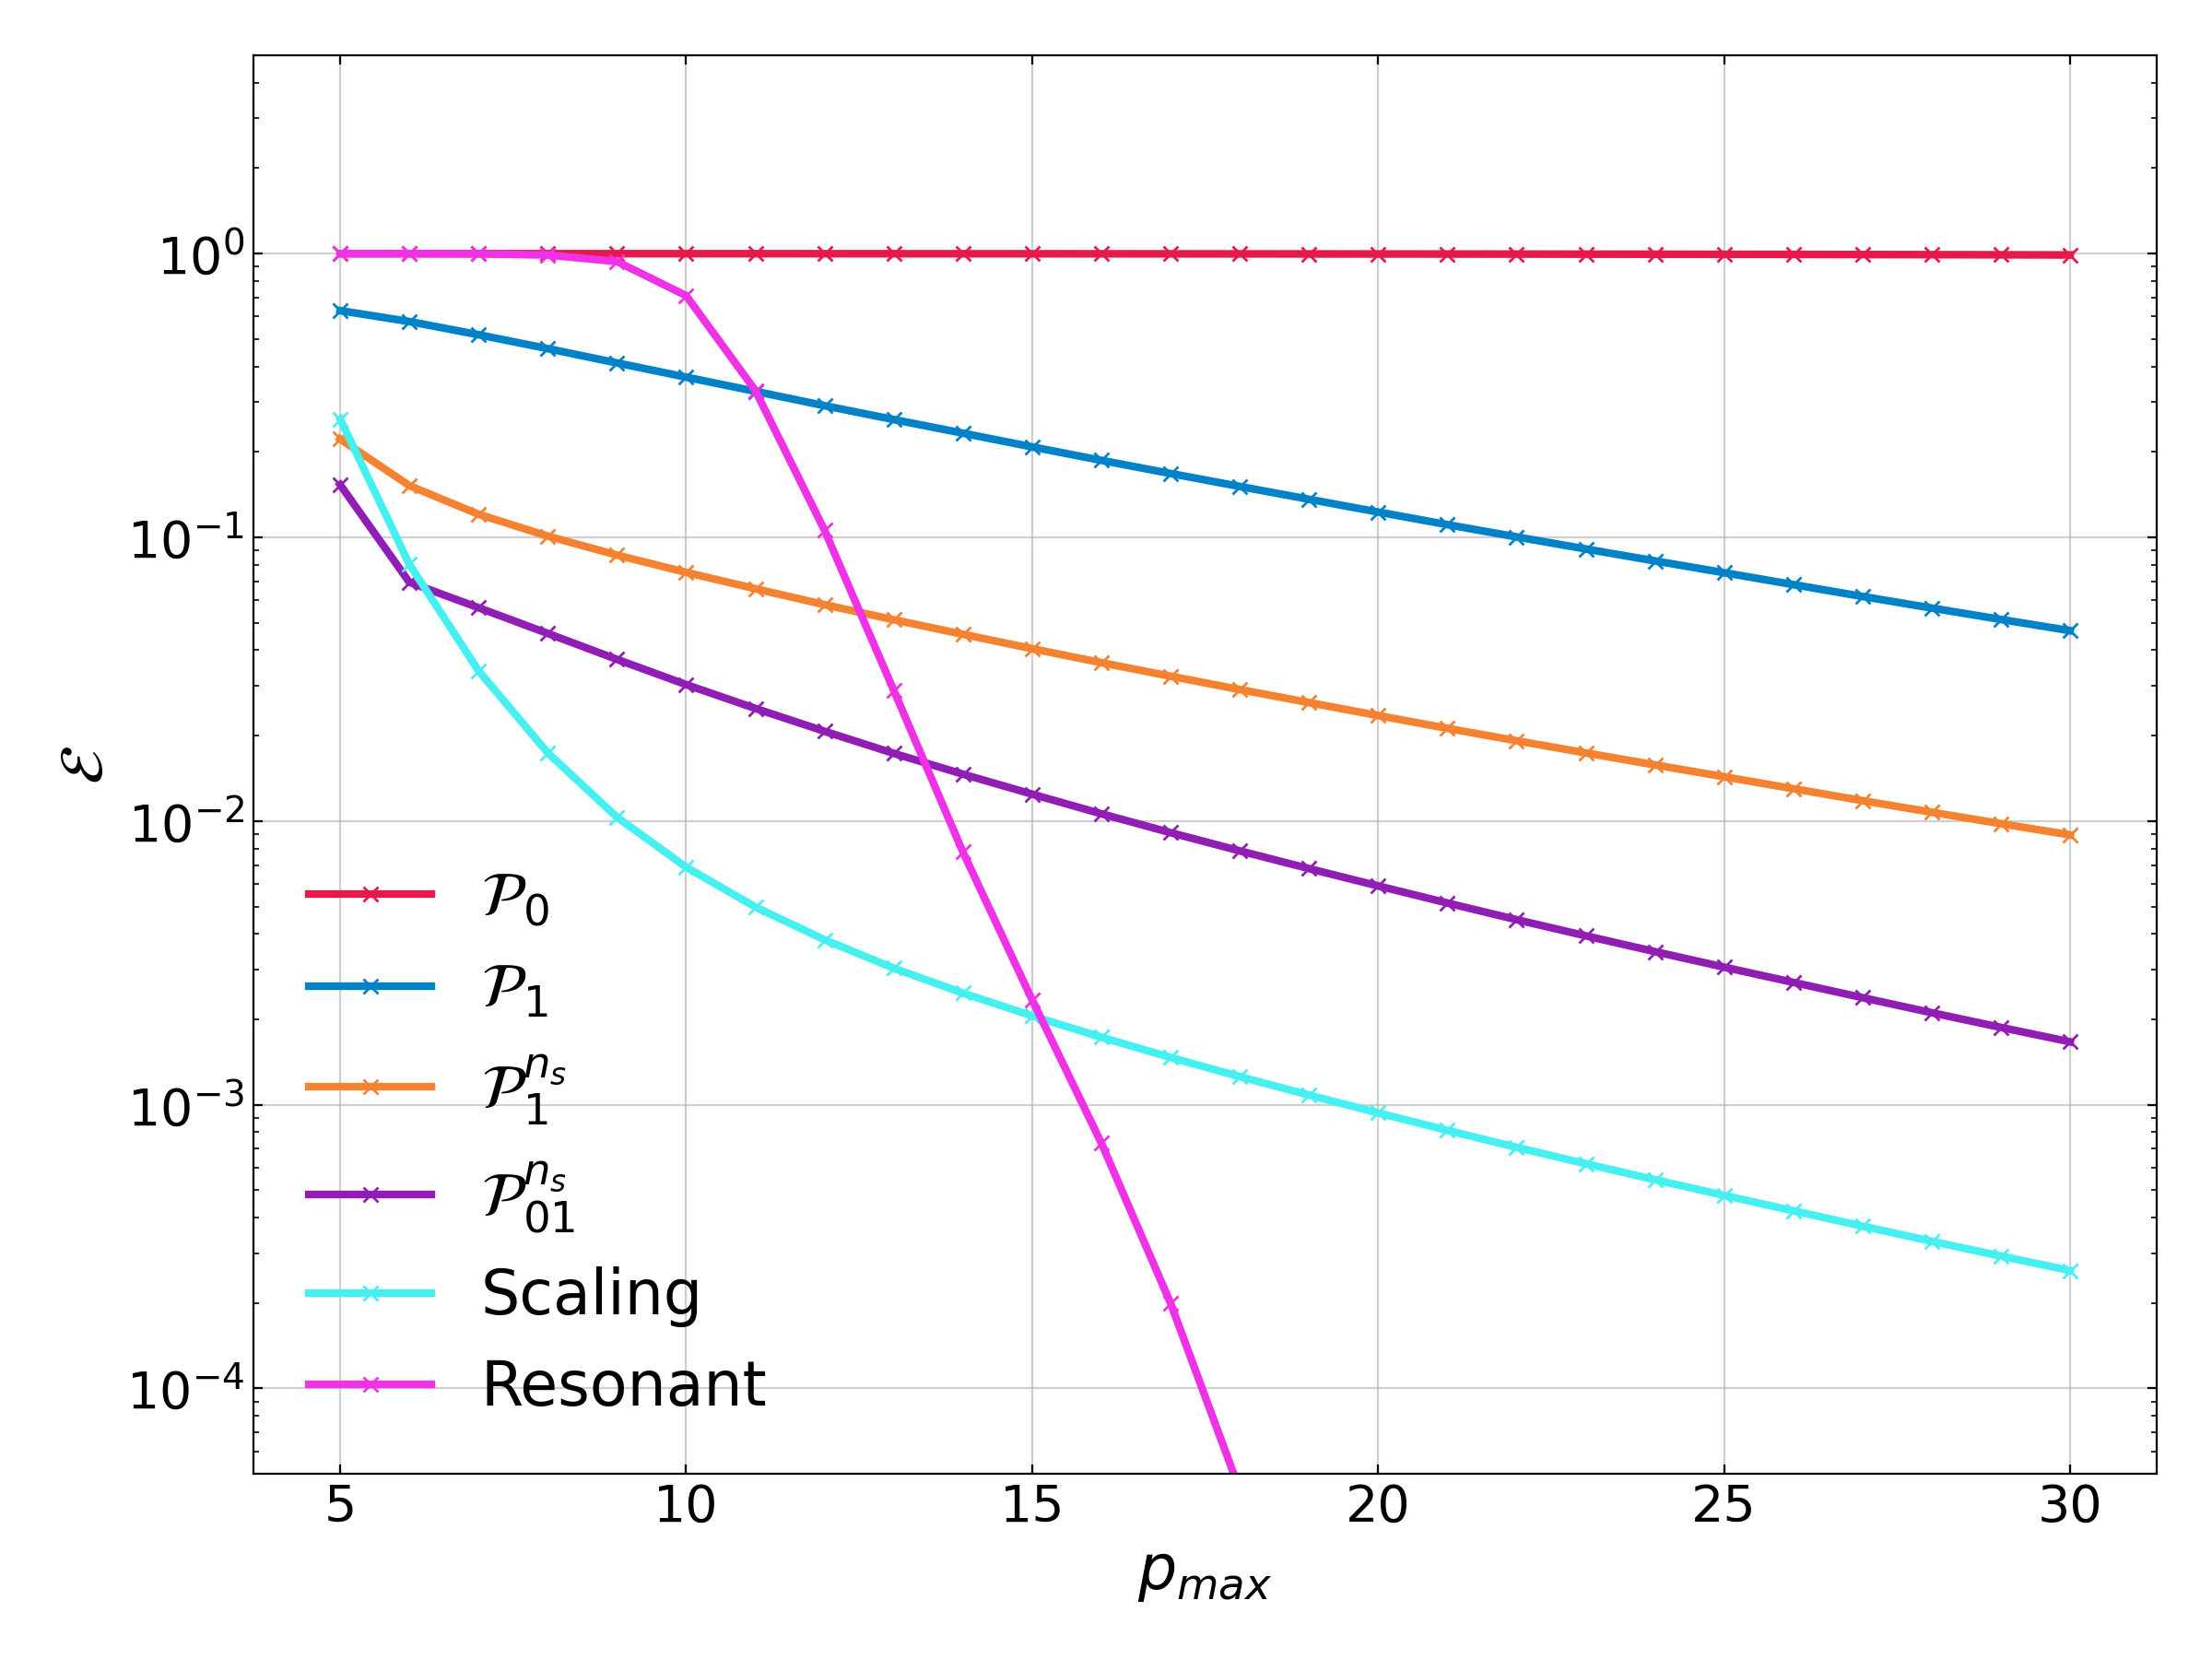
\includegraphics[width=0.8\columnwidth]{pmax_reduction_plots_1_1000/dbi_scaling.png}
\subfloat[$\kmax/\kmin=550$]{\label{fig:scale_550}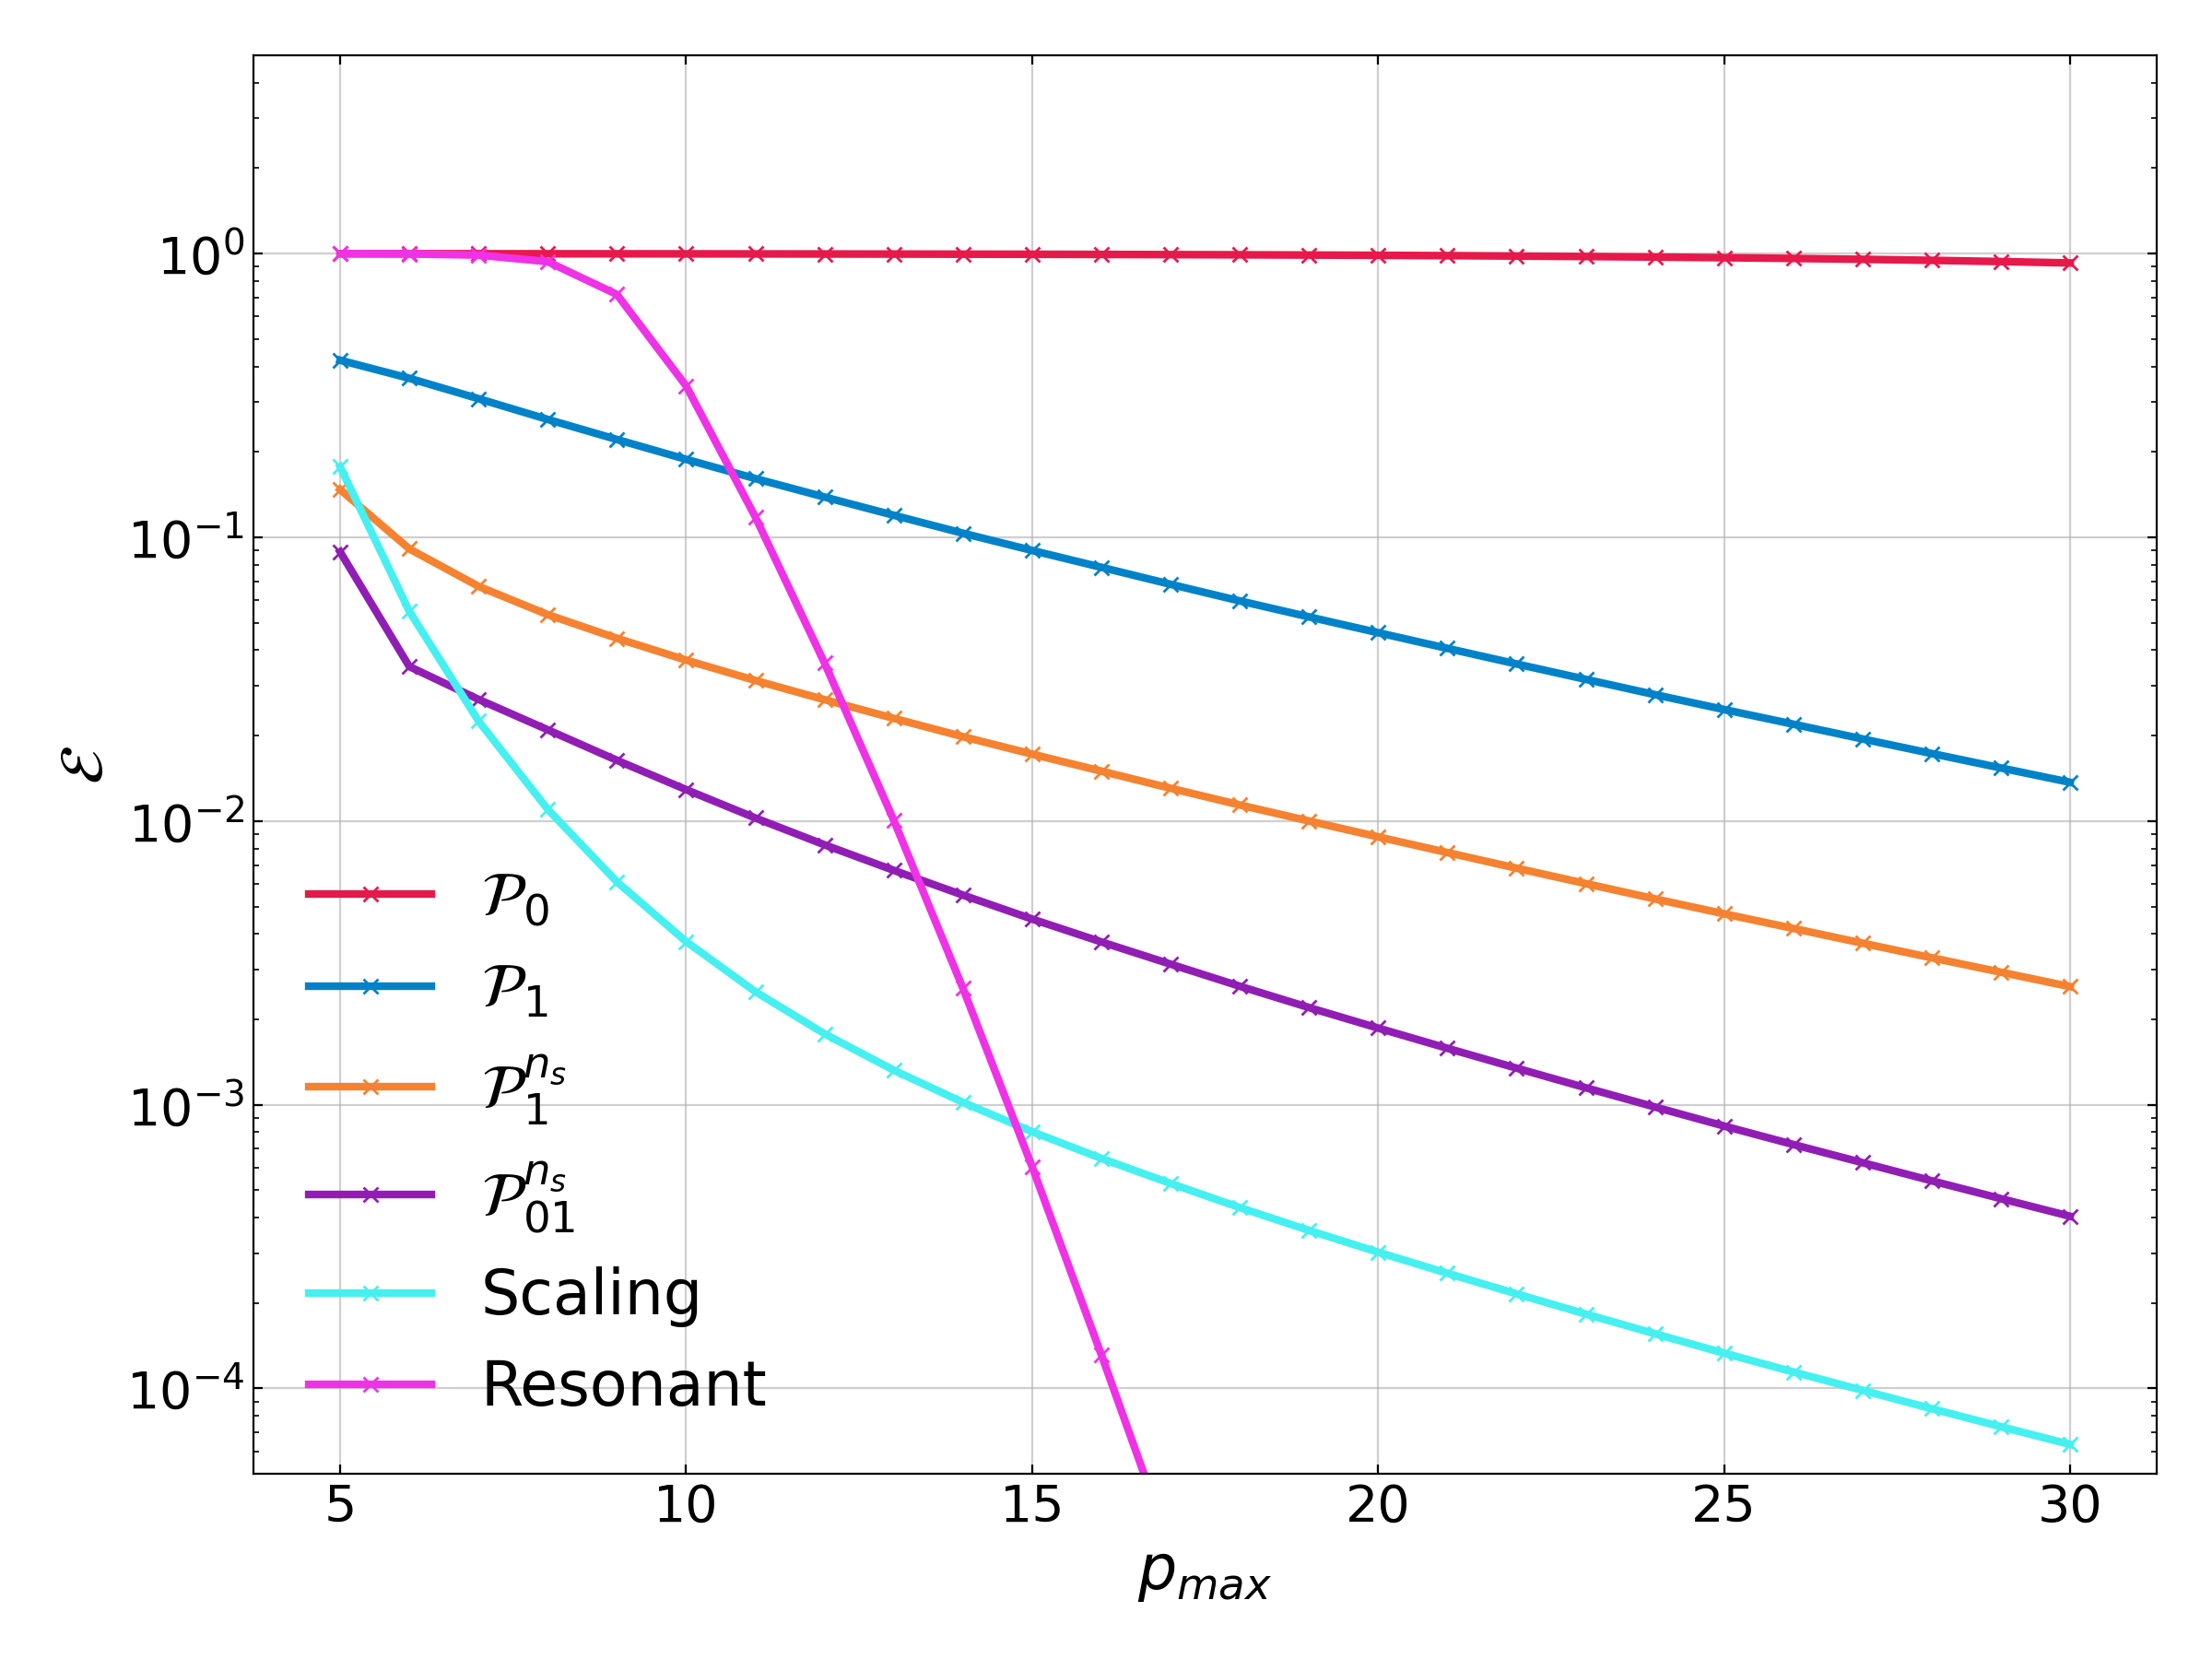
\includegraphics[width=.75\columnwidth]{pmax_reduction_plots_1_550/dbi_scaling.png}}\\
\subfloat[$\kmax/\kmin=1000$]{\label{fig:scale_1000}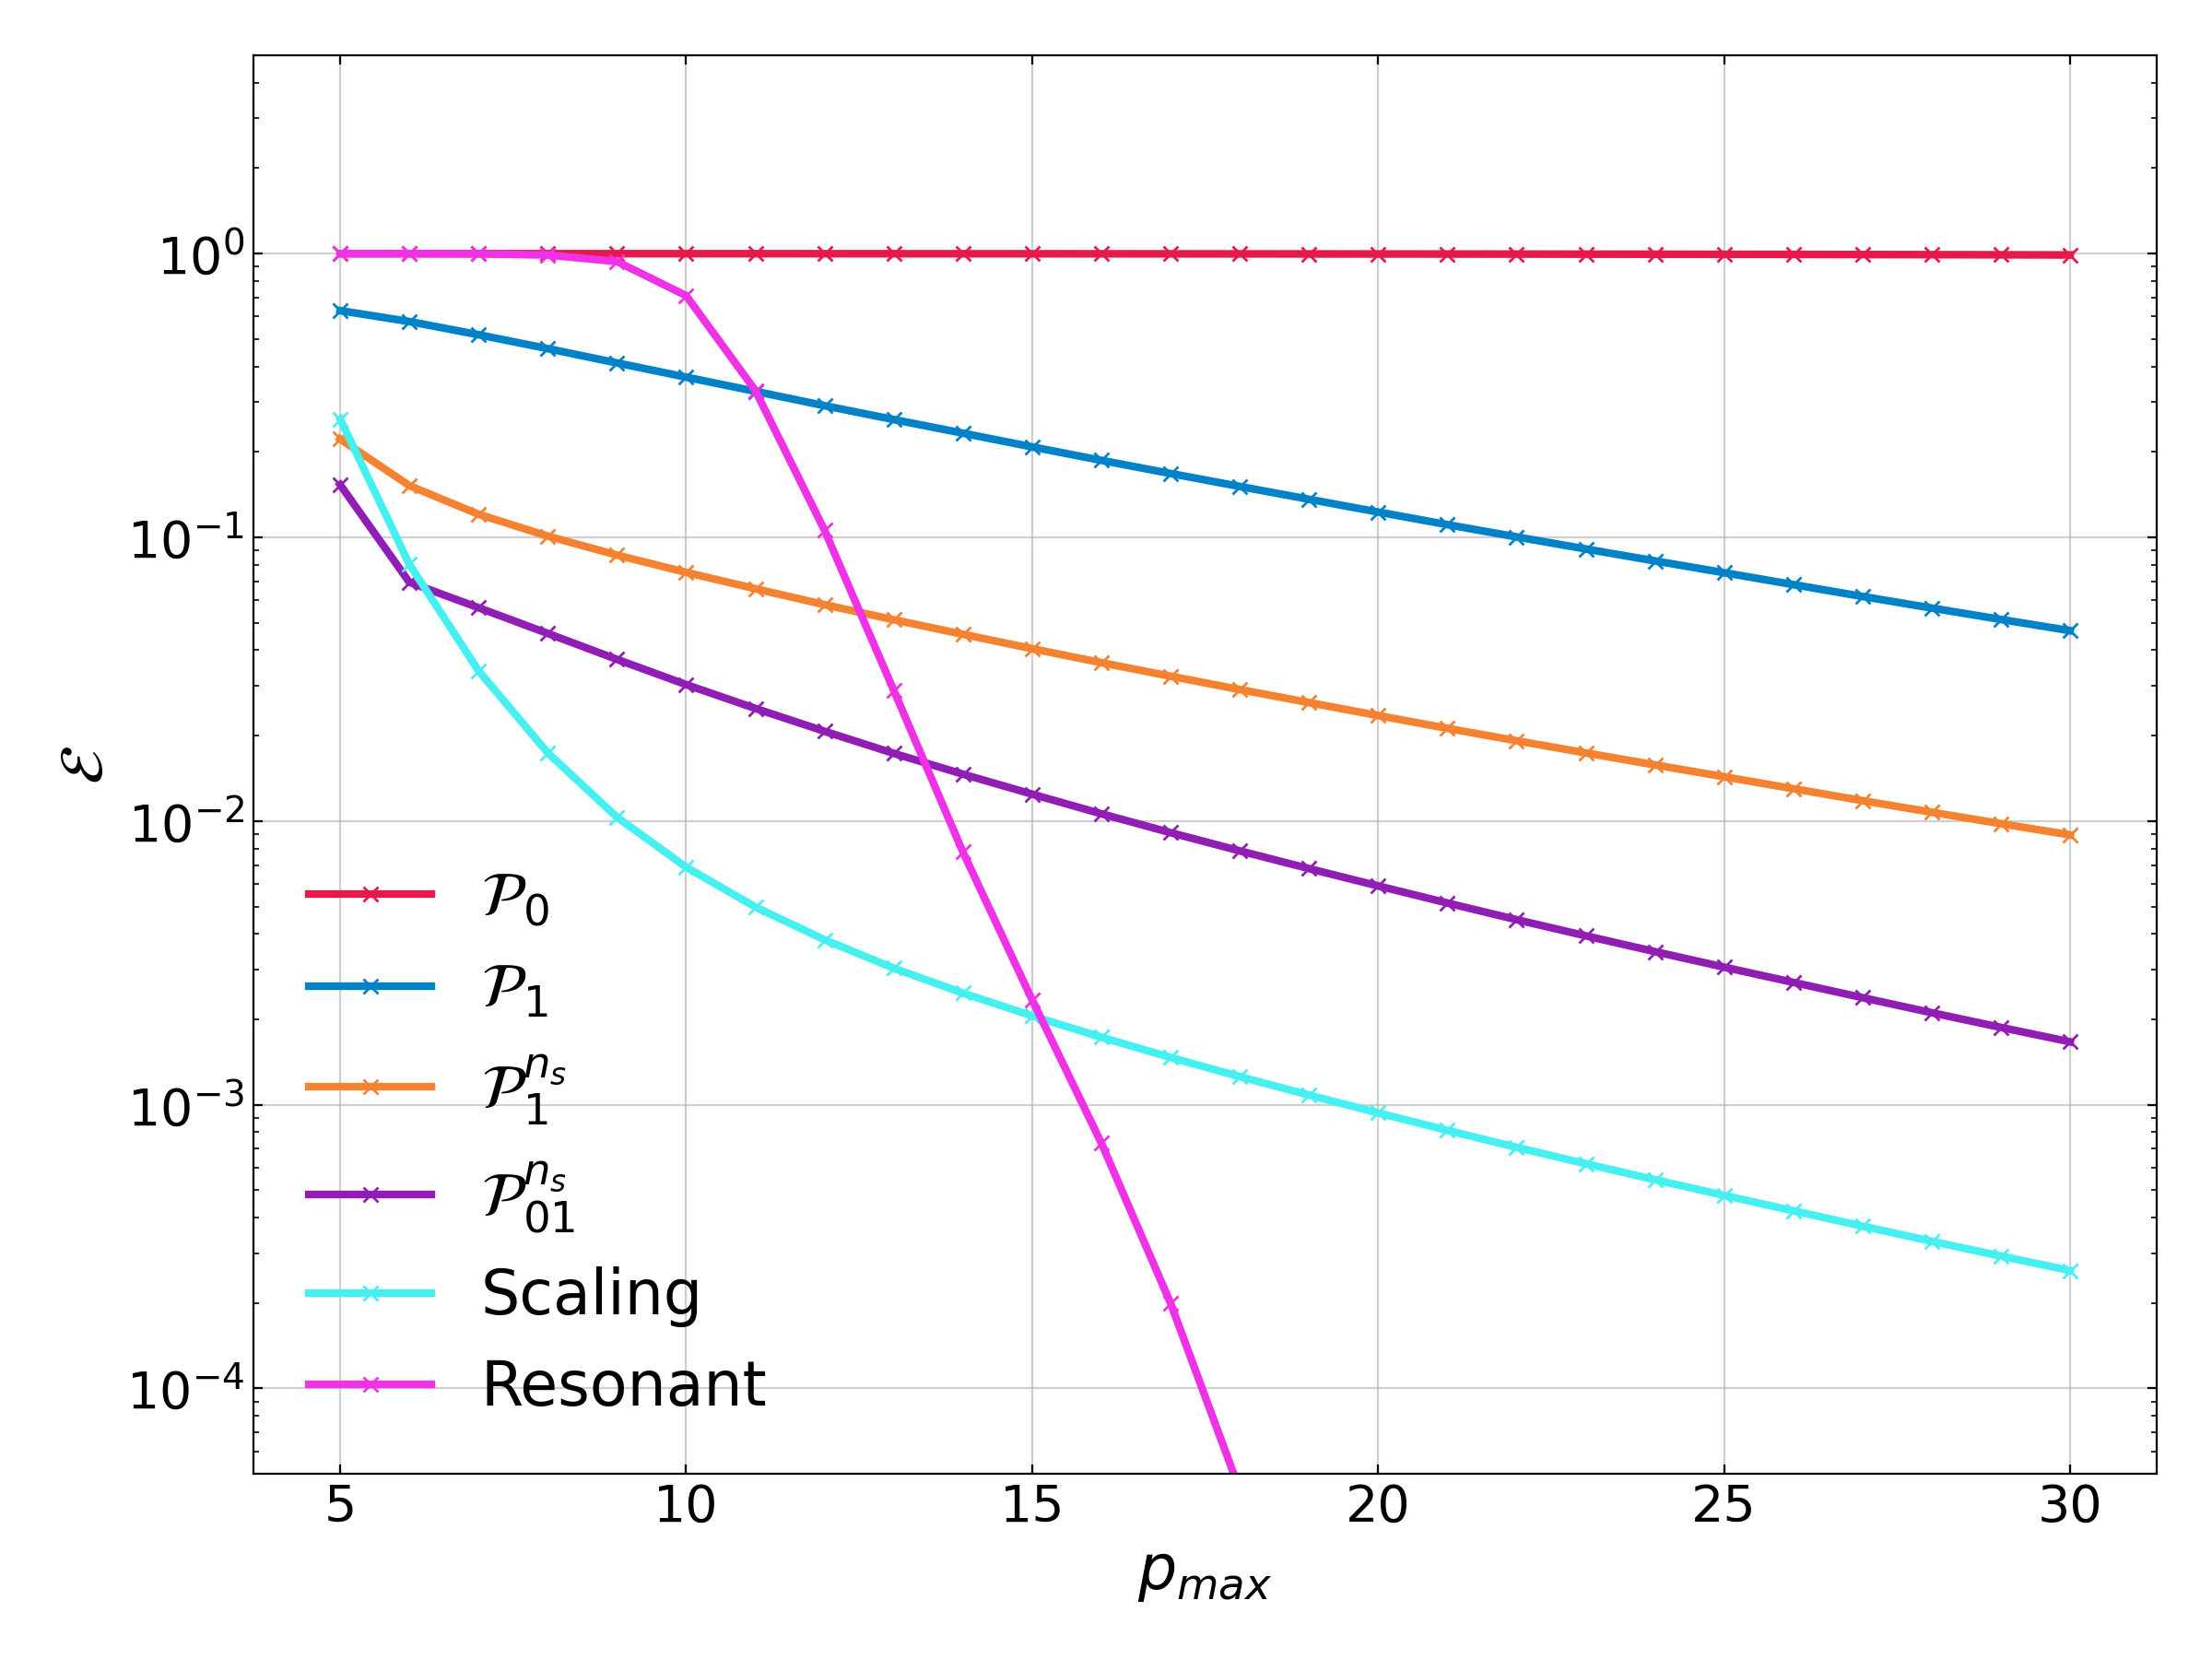
\includegraphics[width=.75\columnwidth]{pmax_reduction_plots_1_1000/dbi_scaling.png}}\\
\caption{
    For the scale-dependent DBI template~\eqref{dbi_prod_shape},
    by including a minimal amount of power spectrum information
    using~\eqref{Lns_inv} and~\eqref{Lns_both} ($\Lnsinv$ with
    $n_s^{*}=0.9649$), we can decrease the convergence error
    by nearly an order of magnitude (compared to $\Linvk$), reaching sub-percent errors at $\Pmax=30$.
    The $\scalingbasis$ basis performs far better again, even without the extra
    power spectrum information.
    By far the fastest convergence, however, results from the $\resobasis$ basis.
    The convergence of this template also has a dependence on $\kmax/\kmin$.
    The convergence power of these basis sets will allow us to efficiently
    capture the scale dependence of the numerically calculated shape function.
    }\label{fig:recon_dbi_ns}
\end{figure}

\begin{figure}[!pth]
\centering
\subfloat[$\cos(\omega(k_1+k_2+k_3))$]{\label{fig:freq_a}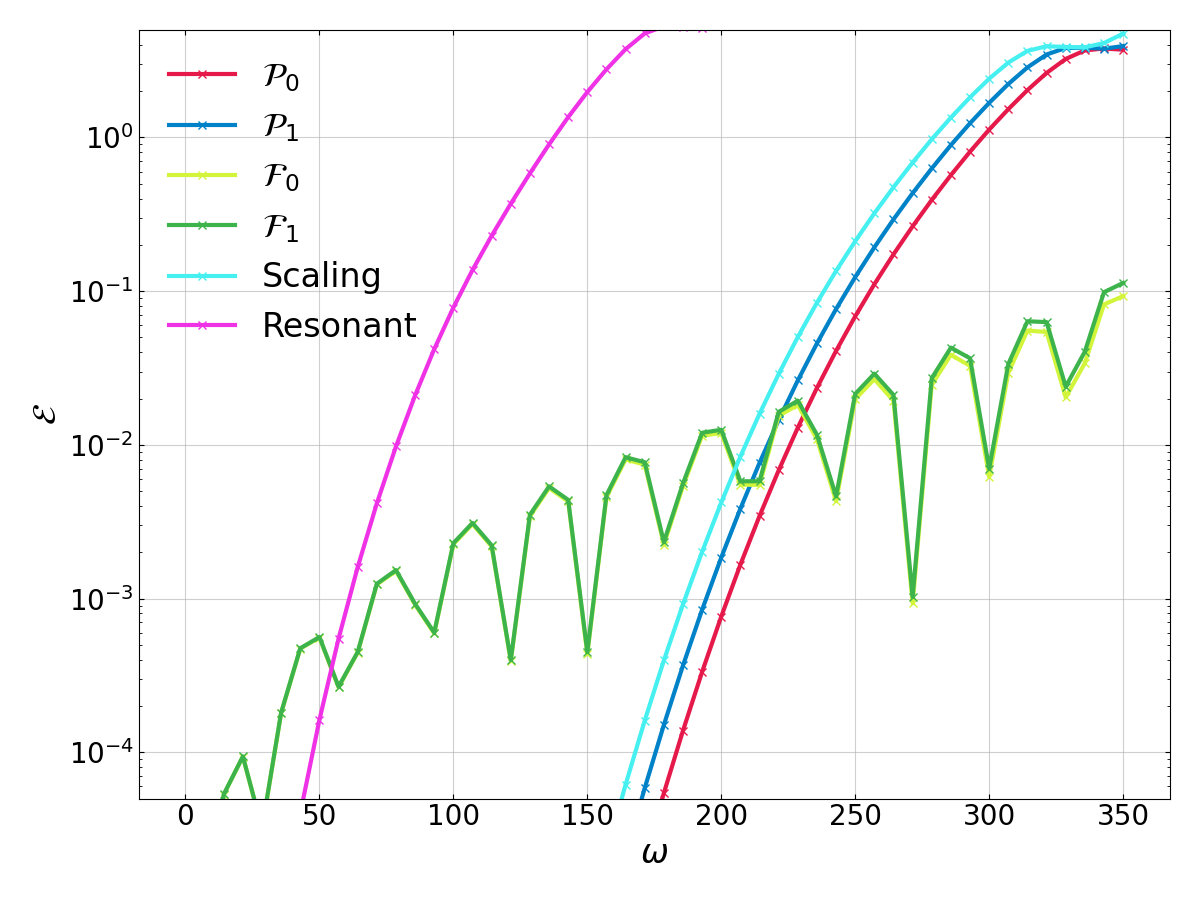
\includegraphics[width=.75\columnwidth]{freq_scan_plots/cos_freq_scan.png}}\\
\subfloat[$\cos(\omega\ln(k_1+k_2+k_3))$]{\label{fig:freq_b}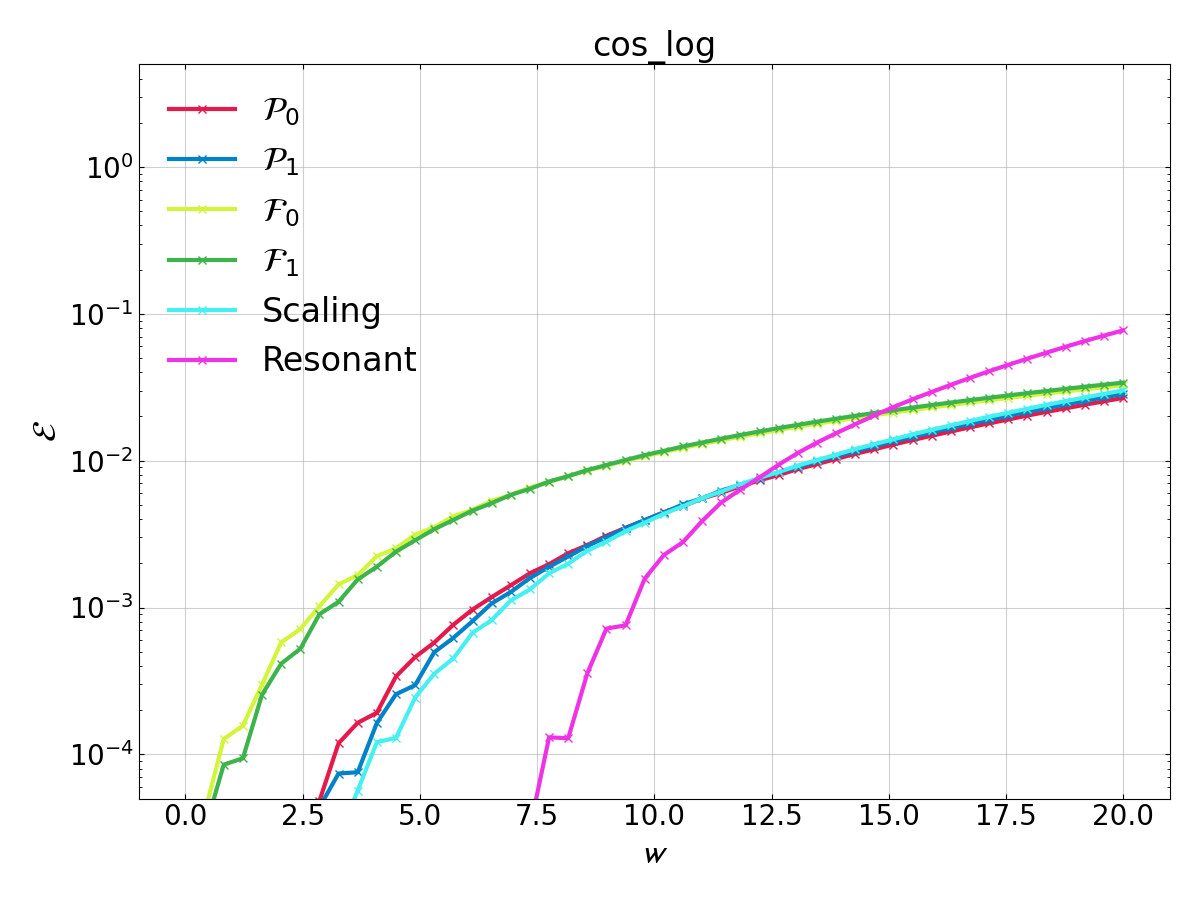
\includegraphics[width=.75\columnwidth]{freq_scan_plots/cos_log_freq_scan.png}}\\
\caption{
    Here we test our basis sets on oscillatory templates, which are a good proxy for feature models.
    These plots are useful to aid in deciding which basis to run $\cmbbest$ for,
    in determining which covers the widest range of features.
    The $\Lnsinv$ basis is not included in every plot, but would always perform between
    the $\Lbasic$ and $\scalingbasis$ basis.
    The basis sets are defined in table~\ref{tab:basis_summary},
    and some are plotted in figures~\ref{fig:basis_pmax5_plots_a}
          and~\ref{fig:basis_pmax5_plots_b}.
    Basis sets~$\Linvk$ and $\scalingbasis$ work well for the linear oscillations,
    converging up to around $\omega\approx200$.
    For logarithmic oscillations the resonant basis works best, as expected.
    However, the improvement is less dramatic.
    }\label{fig:plot_freq_scan}
\end{figure}
\begin{figure}[!pth]
\centering
\subfloat[$\cos(\omega(k_1+k_2+k_3))S^{DBI}$]{\label{fig:freq_c}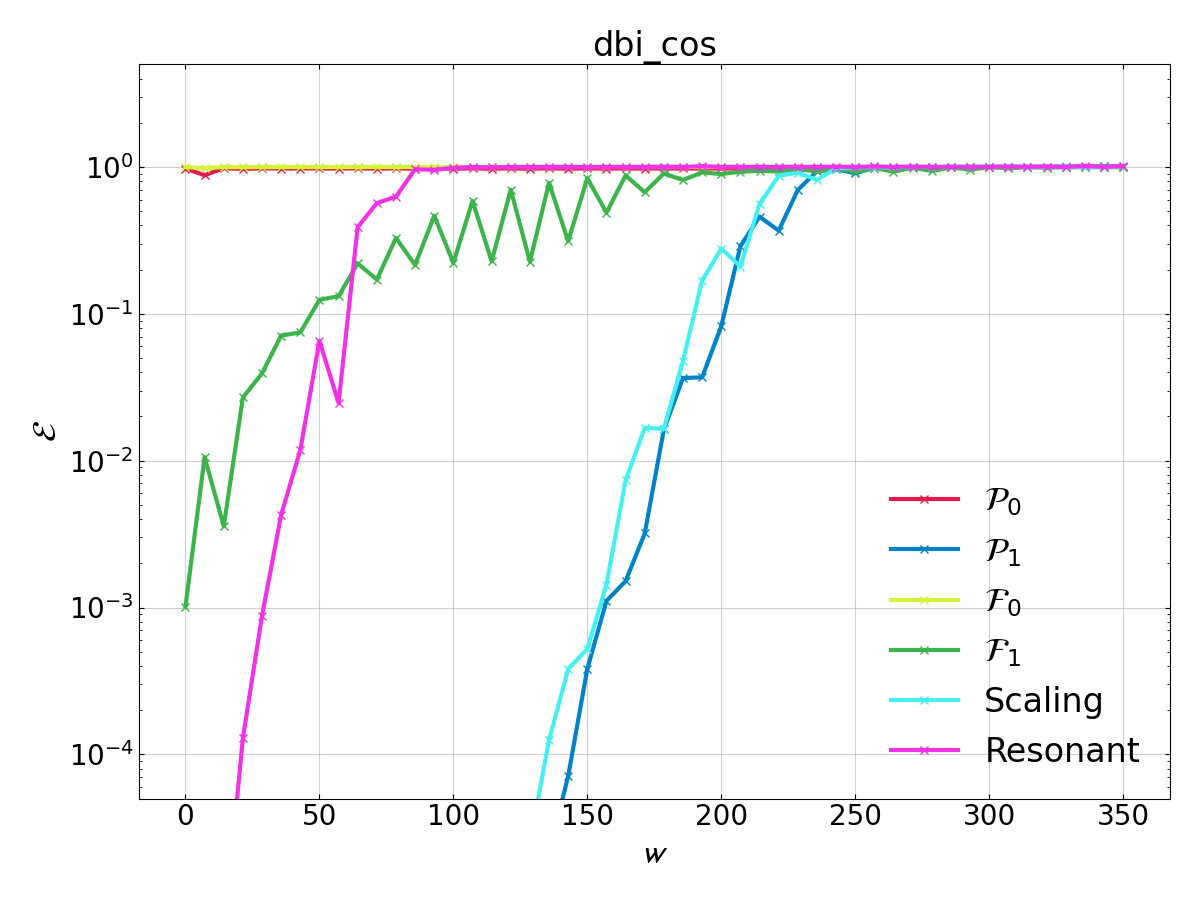
\includegraphics[width=.75\columnwidth]{freq_scan_plots/dbi_cos_freq_scan.png}}\\
\subfloat[$\cos(\omega\ln(k_1+k_2+k_3))S^{DBI}$]{\label{fig:freq_d}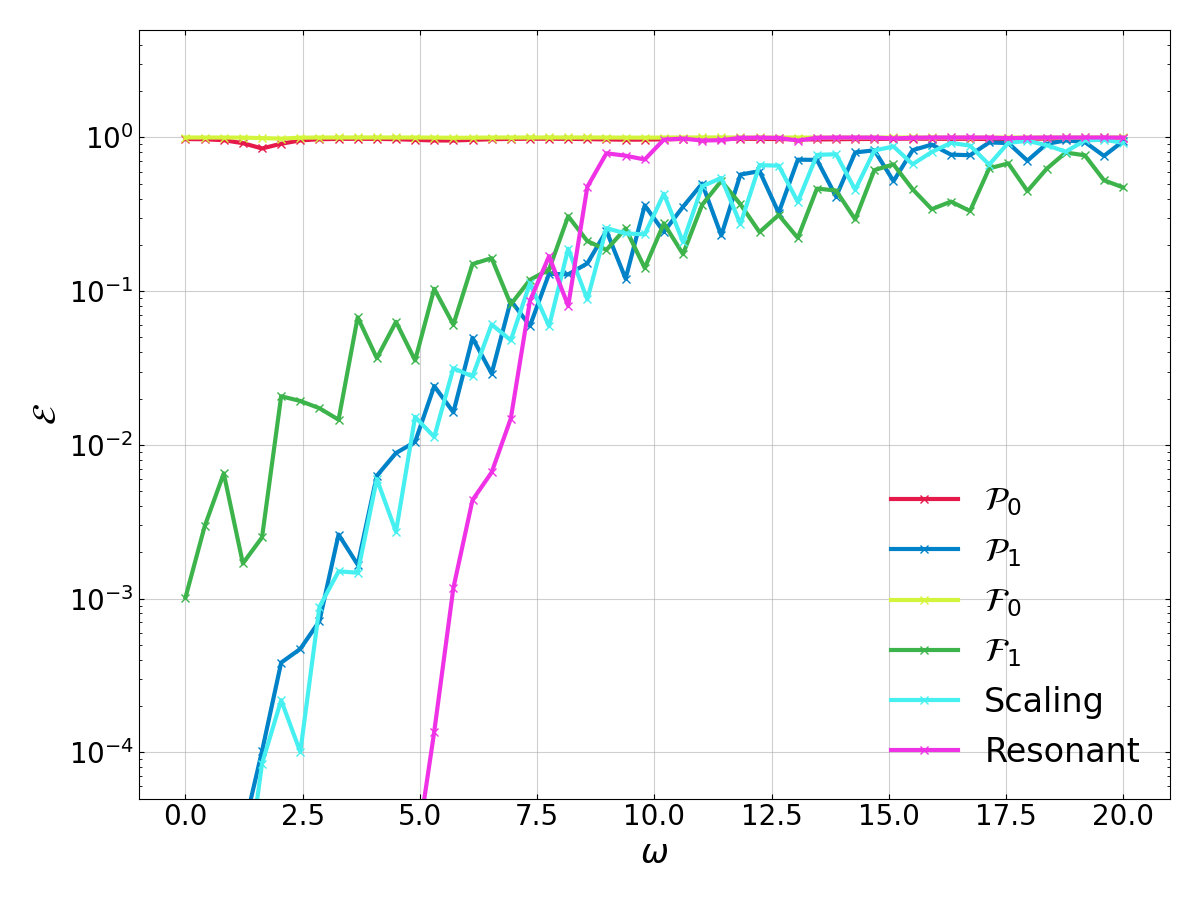
\includegraphics[width=.75\columnwidth]{freq_scan_plots/dbi_cos_log_freq_scan.png}}\\
\caption{
    We hold the basis size $\Pmax$ fixed at $30$ and increase the frequency of
    the oscillatory template.
    For linear oscillations with non-trivial shape dependence (a) we see that
    $\Lnsinv$ and the $\scalingbasis$ basis converge for a significantly larger
    frequency range than the $\resobasis$ basis, as expected.
    We also see that $\Fbasic$ and $\Finvk$ converge very poorly due to the
    DBI shape, only covering around a tenth of the frequency range that
    the $\scalingbasis$ basis converges for, up to $\omega\approx170$.
    For logarithmic oscillations the resonant basis converges best,
    capturing the complex oscillatory templates up to around $\omega\approx7$.
    Beyond this point none of the basis sets converge so the relative
    performance is irrelevant, but we can see that the $\resobasis$ basis
    actually has the largest error in this region---this is due to that basis
    being constructed out of orthogonal Legendre polynomials with
    a log-scaled argument.
    }\label{fig:plot_freq_scan_dbi}
\end{figure}

Finally, we consider convergence in the light of the more subtle scale-dependence due to
the spectral index $n_s$ of the power spectrum.
The simple canonical examples in figure~\ref{fig:recon_malda_dbi} had shape dependence and no scale dependence,
but this would only be expected of scenarios unrealistically deep in the slow-roll limit.
When we include this scale dependence, using~\eqref{dbi_prod_shape} with $n^*_s$, 
it proves very useful to include these deviations from
integer power laws in the basis functions.  We will now consider two cases, first augmenting
$\Lbasic$ by a scale-dependent $1/k$ term using the orthogonalisation procedure~\eqref{gram_schmidt}, 
\begin{align}\label{Lns_inv}
    q_{\Pmax-1}(k) = \text{Orth}\left[{k^{-1+(n_s^{*}-1)}},~\Lbasic\right],
\end{align}
which we refer to as $\Lnsinv$.
Secondly, we instead augment $\Lbasic$ with an additional scale-dependent terms
\begin{align}\label{Lns_both}
    %q_{\Pmax}(k) = \text{Orth}\left[{k^{(n_s^{*}-1)}},~\Lbasic\right],\qquad  q_{\Pmax\text{$+$}1}(k) = \text{Orth}\left[{k^{-1+(n_s^{*}-1)}},~\Lbasic\right],
    {k^{(n_s^{*}-1)}},\qquad{k^{-1+(n_s^{*}-1)}}
\end{align}
which we refer to as $\Lnsboth$.


    It is worth noting that while $\Lbasic$ with (e.g.) $\Pmax=20$ is a subset of
    $\Lbasic$ with any higher $\Pmax$, $\Lnsinv$ with (e.g.) $\Pmax=20$ is not a subset of
    $\Lnsinv$ with any higher $\Pmax$ as the augmented term will be orthogonalised
    with respect to a different set of functions.


As we see in figure~\ref{fig:recon_dbi_ns}, for equilateral type shapes
even a small overall scale dependence causes significant degradation in the convergence of
the original augmented Legendre basis $\Linvk$.
However, incorporating the spectral index $n_s$  into the basis functions $\Lnsinv$ and $\Lnsboth$
results again in rapid convergence to the scale-dependent DBI template, which can then be accurately
approximated with a limited number of modes.
We conclude using power spectrum information to augment the basis functions with terms incorporating the expected dependence
on the spectral index enables the efficient approximation of high precision primordial bispectra.
This is still not optimal, however, as the scaling of the bispectrum is not uniquely defined by the
scaling of the power spectrum, so more flexibility would be desirable---we will explore this further
in section~\ref{sec:scaling_definition}.


\section{The $\scalingbasis$ basis}\label{sec:scaling_definition}
    Despite having the same power spectrum scaling,
    different models can have different bispectrum scalings.
    Therefore while the power spectrum can give us a
    rough estimate of the scaling of the bispectrum,
    the $\Lnsinv$ basis may not converge sufficiently quickly if~\eqref{Lns_inv}
    is not a sufficiently close match to the required scaling.
    We would instead like a basis that could fit
    a range of fractional powers of $k$.
    We achieve this using the $\scalingbasis$ basis.
    The $\scalingbasis$ basis is built using the Legendre polynomials,
    augmented (in the sense of~\eqref{gram_schmidt})
    with
    \begin{align}\label{scaling_basis_definition}
        k^{-1},\qquad \ln(k)k^{-1}
        %q_{\Pmax-2}(k) &= \text{Orth}\left[{k^{-1}},~\Lbasic\right],\\
        %q_{\Pmax-1}(k) &= \text{Orth}\left[{\ln(k)k^{-1}},~\Lbasic\right].
    \end{align}
    This is motivated by
    \begin{align}
        k^\epsilon &= e^{\epsilon\ln\left(\frac{k}{\kmin}\right)+\epsilon\ln(\kmin)}\\
                   &\approx e^{\epsilon\ln\left(\kmin\right)}
                      \left(1+\epsilon\ln\left(\frac{k}{\kmin}\right)\right)
    \end{align}
    which is valid when $\epsilon\ln\left(\kmax/\kmin\right)$ is
    sufficiently small.
    Since for the DBI case the scaling exponent $\epsilon$ is expected to be of the
    same order as $n_s-1$ and $\varepsilon_s$, we see that this
    approximation is good for our case,
    where (as we will discuss in section~\ref{sec:tradeoff})
    we have $\ln\left(\frac{\kmax}{\kmin}\right)\approx6.91$.
    By adding $k^{-1}$ and $\ln(k)k^{-1}$ separately to our
    basis, their relative coefficient will be set to the value
    which provides the best fit to the final shape,
    providing the flexibility needed to fit shapes with different
    scalings with the same basis, so we have no need to know anything
    about the scaling a priori (except that it is small).


    For the feature templates, for example figure~\ref{fig:plot_freq_scan},
    we see that the $\scalingbasis$ basis performs equivalently to $\Lnsinv$
    and $\Lbasic$.
    This is because these template have no scaling or complex shape dependence,
    and the fit to the oscillatory feature is due to the Legendre polynomials
    in the basis.
    In figure~\ref{fig:plot_freq_scan_dbi} we see that the $1/k$ behaviour is
    necessary to achieve an acceptable fit, but since these templates
    do not need non-integer scaling, the $\scalingbasis$ basis performs
    equivalently to $\Linvk$, as expected.


    As we can see in figure~\ref{fig:recon_dbi_ns} however, the $\scalingbasis$ basis
    converges quickly to a DBI template with a realistic scaling. It outperforms
    the $\Lnsinv$ basis, despite not assuming power spectrum information.

\section{The $\resobasis$ basis}\label{sec:resobasis_definition}
    We finally describe a basis specifically designed to capture logarithmic oscillations,
    a type of feature that is usually very difficult to accurately fit.
    This goes against our philosophy of desiring a basis that is not tied to
    any specific shape, which was motivated by the fact that $\cmbbest$
    is expensive but need only be run once per basis.
    However, logarithmic oscillations are an important type of feature in the
    literature~\cite{Planck_NG_2018}.
    Running $\cmbbest$ twice, once for a basis that can cover
    a broad range of general features, and once for
    logarithmic oscillations in particular,
    may be a viable strategy to cover a very broad range of models.


    The $\resobasis$ basis is built using the Legendre polynomials,
    however the argument has been scaled logarithmically.
    It differs from the basis described in~\cite{Funakoshi} in that it
    also includes a factor of $\frac{1}{\sqrt{k}}$ to retain orthogonality.
    We define the $n$th basis element as
    \begin{align}
        \frac{\mathcal{P}_n(\bar{k})}{\sqrt{k}}\text{,}\qquad \bar{k}=\frac{2\ln(k)-\ln(\kmin\kmax)}{\ln(\kmax)-\ln(\kmin)}.
    \end{align}\label{reso_basis_definition}
    We then see that
    \begin{align}
        \int_{\kmin}^{\kmax}dk\frac{\mathcal{P}_m(\bar{k})}{\sqrt{k}}\frac{\mathcal{P}_n(\bar{k})}{\sqrt{k}}
        = \int_{\ln\kmin}^{\ln\kmax}d\ln{k}~\mathcal{P}_m(\bar{k})\mathcal{P}_n(\bar{k})
        \propto \delta_{mn}
    \end{align}
    so the $\resobasis$ basis is orthogonal
    due to the way we defined $\bar{k}$ for this basis set.

    In figure~\ref{fig:plot_freq_scan} we see that for linear oscillations, as expected,
    the $\resobasis$ basis converges for a much smaller range for frequencies
    (for fixed basis set size $\Pmax=30$) than the other basis sets we test.
    For logarithmic oscillations however, we see that the range of accessible
    frequencies is nearly doubled when compared to the other basis sets.
    We also note that for logarithmic oscillations,
    wherever we have acceptable convergence the $\resobasis$ basis converges best.
    We also see however that in the frequency range where none of our basis sets
    converge, the $\resobasis$ basis has the largest error. This is because
    the $\resobasis$ basis is designed to be a set of orthogonal logarithmic
    oscillations, and so will be orthogonal to frequencies outside of its range.
    On the other hand, while the $\scalingbasis$ basis (for example) has
    a worse fit for lower frequencies, it has a better fit to higher frequencies as
    it is not orthogonal to them. We emphasise however that this only occurs
    in the region where none of our basis sets provide acceptable convergence
    for $\Pmax=30$.

    We also note the surprising result in figure~\ref{fig:recon_dbi_ns}
    that the $\resobasis$ basis performs best at converging to the
    scale-dependent DBI template. However, the convergence of the
    $\scalingbasis$ basis is still perfectly adequate in this case.
    \begin{figure}[!pth]
        \centering
        \subfloat[$\Lbasic$]{\label{fig:basis_plot_a}\includegraphics[width=.85\columnwidth]{basis_plot_diagrams/basis_pmax5_plot_P_0}}\\
        \subfloat[$\Linvk$]{\label{fig:basis_plot_b}\includegraphics[width=.85\columnwidth]{basis_plot_diagrams/basis_pmax5_plot_P_1}}\\
        \subfloat[$\scalingbasis$ basis]{\label{fig:basis_plot_e}\includegraphics[width=.85\columnwidth]{basis_plot_diagrams/basis_pmax5_plot_scaling}}\\
        \caption{
            We plot the $\Lbasic$, $\Linvk$ and $\scalingbasis$ basis sets from
            table~\ref{tab:basis_summary}, for $\Pmax=5$. Note that these sets
            have Legendre polynomial basis elements in common, but differ in
            which functions they are augmented by, which are added to the start of the
            indexing.
        }\label{fig:basis_pmax5_plots_a}
    \end{figure}
    \begin{figure}[!pth]
        %\ContinuedFloat
        \centering
        \subfloat[$\Fbasic$]{\label{fig:basis_plot_c}\includegraphics[width=.85\columnwidth]{basis_plot_diagrams/basis_pmax5_plot_F_0}}\\
        \subfloat[$\Finvk$]{\label{fig:basis_plot_d}\includegraphics[width=.85\columnwidth]{basis_plot_diagrams/basis_pmax5_plot_F_1}}\\
        \subfloat[$\resobasis$ basis]{\label{fig:basis_plot_f}\includegraphics[width=.85\columnwidth]{basis_plot_diagrams/basis_pmax5_plot_reso}}\\
        \caption{
            We plot the $\Fbasic$, $\Finvk$ and $\resobasis$ basis sets from
            table~\ref{tab:basis_summary}, for $\Pmax=5$. Note that
            $\Fbasic$ and $\Finvk$
            have Fourier basis elements in common, but differ in
            which functions they are augmented by. The $\resobasis$ basis
            differs in all of its basis elements, lacking even
            a constant basis element due to the factor of
            $1/\sqrt{k}$ added to retain orthogonality.
        }\label{fig:basis_pmax5_plots_b}
    \end{figure}


\subsection{Large non-physical contributions}\label{large_non_physical}
    When a shape is dominated by its non-physical configurations
    (those that do not obey the triangle inequality~\eqref{triangle_inequality})
    then we can see slow convergence on the tetrapyd, despite
    possibly fast convergence on the cube as a whole.
    We will refer to convergence on the tetrapyd as $\totalcortet$
    and the convergence on the cube as $\totalcorcub$.
    For a pure oscillation we see no significant difference between the convergence on the cube
    and on the tetrapyd, as expected for a shape where the physical and non-physical
    configurations are of the same order of magnitude.
    For an oscillation with a DBI shape however, we see a large difference,
    as shown in figure~\ref{fig:log_recon_osc_dbiosc}.
    On the cube we see fast, monotonic convergence---the $\resobasis$ basis
    and $\scalingbasis$ basis perform well, quickly bring $\totalcorcub$
    below $0.1\%$.
    On the tetrapyd however, we see that $\totalcortet$ only drops below
    $0.1\%$ for $\Pmax<30$ for the $\resobasis$ basis.


    We also see that the improvement in $\totalcortet$ is no longer
    monotonic, there are regions where increasing $\Pmax$ results in
    a larger $\totalcortet$.
    To understand this it is important to remember that we are not simply
    adding modes as we increase $\Pmax$---the augmented mode is changing
    each time, and thus while we expect $\totalcorcub$ to decrease monotonically,
    there is no such guarantee for point-wise convergence.


    We also notice that $\totalcortet$ stays fixed at $1$ for low values of $\Pmax$.
    This is due to the basis fitting the large non-physical configurations,
    and thus in~\eqref{relative_difference}, $S_2 \gg S_1$ everywhere on the cube.


    For the local shape the mean value of the shape function on the entire cube
    (thus accounting for volume effects) is approximately a factor of $40$ larger than the mean
    when restricted to the tetrapyd. For the equilateral template, this factor becomes $-300$.
    This illustrates why the tetrapyd-vs-cube problem is so much more severe for equilateral-type
    shapes than for local shapes, as the non-physical configurations are an order of magnitude
    more dominant.


    This phenomenon is a major obstacle to preserving the separability of the in-in formalism,
    due to the restriction that we must (effectively, if not in a literal sense) fit to the cube---we
    have seen that neglecting it and using a simple basis such as $\Lbasic$ would be disastrous.
    However, as we have seen, the more sophisticated basis sets described in this chapter are capable
    of overcoming this obstacle, without surrendering generality.

\section{A tradeoff between $\Pmax$ and $\kmax/\kmin$}\label{sec:tradeoff}
    While it may not be intuitively apparent, the value of $\kmax/\kmin$
    affects convergence even in the absence of significant features.
    We can see this in figure~\ref{fig:recon_dbi_ns}.
    In this figure we plot the convergence of various basis sets for the scale-dependent
    DBI template~\eqref{dbi_prod_shape}, for $\kmax/\kmin=550$ and
    for $\kmax/\kmin=1000$. We see that the convergence is slower
    for higher $\kmax/\kmin$. This means that to achieve the same convergence
    for this shape for a higher $\kmax/\kmin$, we must also go to a higher $\Pmax$.
    For example, if one wanted to achieve an accuracy of $0.1\%$ for this shape
    with the $\scalingbasis$ basis,
    one would need $\Pmax=15$ for $\kmax/\kmin=550$
    and $\Pmax=20$ for $\kmax/\kmin=1000$
    We also see this effect for the scale-invariant DBI shape~\eqref{dbi_shape}
    but it significantly less dramatic.


    We of course desire to use as much of the available data as we can.
    As such, it is desirable to have the largest possible $k$-range.
    However, as we can see, this must be weighted against the loss
    of descriptive power, as we will then have a smaller set of shapes which
    will converge sufficiently well to be constrained.


    As described in~\cite{Sohn_2021}, if too much of the squeezed limit is lost,
    constraining power on models such as those of the local type is lost (at the $\cmb$ level).
    It is shown in that work that $\kmax/\kmin=1000$ is sufficient, and as we have seen in this chapter
    this value still retains convergence on a range of interesting models at the primordial level.


%\section{Factor basis?}
%    Words~\cite{tensor_decomp_review}.
%\section{Higher $\Pmax$}
%    Going beyond $\Pmax=30$.
%    How high can I go, in terms of parameters that can't be compared to Planck?
\section{Conclusions}
    \textcolor{red}{My new basis sets, and their dramatic improvement}
    From the plots presented in this chapter it is clear that the problem of the
    large non-physical off-tetrapyd configurations is vitally important to the feasibility of the
    separable in-in calculation of inflationary bispectra.
    In this setting, where we are effectively forced to fit on the whole cube,
    we find that the basic Legendre polynomials and Fourier series basis sets
    are not sufficient to capture the shapes we hope to constrain.
    However, we found that by augmenting the Legendre polynomials with
    basis functions that could capture $1/k$ behaviour, the convergence
    increased dramatically and the range of shapes that could be constrained by
    this pipeline broadens significantly.


    While $\Lnsinv$ improves significantly over $\Lbasic$ for certain examples,
    as it is tied to a particular scaling it is not as ideal solution for a pipeline which requires
    a single basis that can capture the broadest range of shapes, including different scalings.
    To improve upon this situation, we introduced the $\scalingbasis$ basis, which is augmented by
    terms which allow it more flexibility in capturing the scaling of the shape function,
    despite being built without any power spectrum information.


    We also presented results from the $\resobasis$ basis, a basis set designed to converge well
    for logarithmic oscillations, an important target due to the resonance mechanism.
    While this goes against the philosophy of developing one basis set that converges well across the
    broadest possible range of bispectrum shapes, it may be useful in the alternative way forward of
    performing two runs of $\cmbbest$, i.e.\ doing both the scaling basis (for linear oscillations)
    and the resonant basis (for log oscillations).


Future work, using parafac~\cite{tensor_decomp_review}.


    Now that we have demonstrated the feasibility of the overall method, in the next chapter we will
    present its detailed implementation.
